\documentclass{article}
\usepackage[utf8]{inputenc}
\usepackage[margin=2cm]{geometry}
\usepackage{amsmath}
\usepackage{graphicx}
\usepackage{array}
\usepackage{float} % Include this in your preamble


\title{Introduction to Neuroinformatics}
\author{ETH Zurich}
\date{September 2023}

\begin{document}

\maketitle

\section{Overview}
The first lecture of the Introduction to Neuroinformatics course, taught by Melika Payvand at the University of Zurich and ETH Zurich, provides a foundational understanding of neuroinformatics. The course explores various aspects of information processing in the brain, including the organization of neurons and synapses, neural computations, learning and plasticity, encoding of information, theoretical models, and the engineering of brain-like computers.

\subsection{Course Objectives}
The primary objectives of this course are:
\begin{itemize}
    \item To understand how information is processed in the brain, focusing on neurons, synapses, and the nervous system's organization.
    \item To analyze and describe neural computations from an analytical perspective.
    \item To explore the concepts of learning, plasticity, and information encoding within the brain.
    \item To study theoretical neural network models and their applications.
    \item To delve into the development of engineering solutions that mimic brain functions.
\end{itemize}

\subsection{Brain and Information Processing}

\begin{figure}[H]
    \centering
    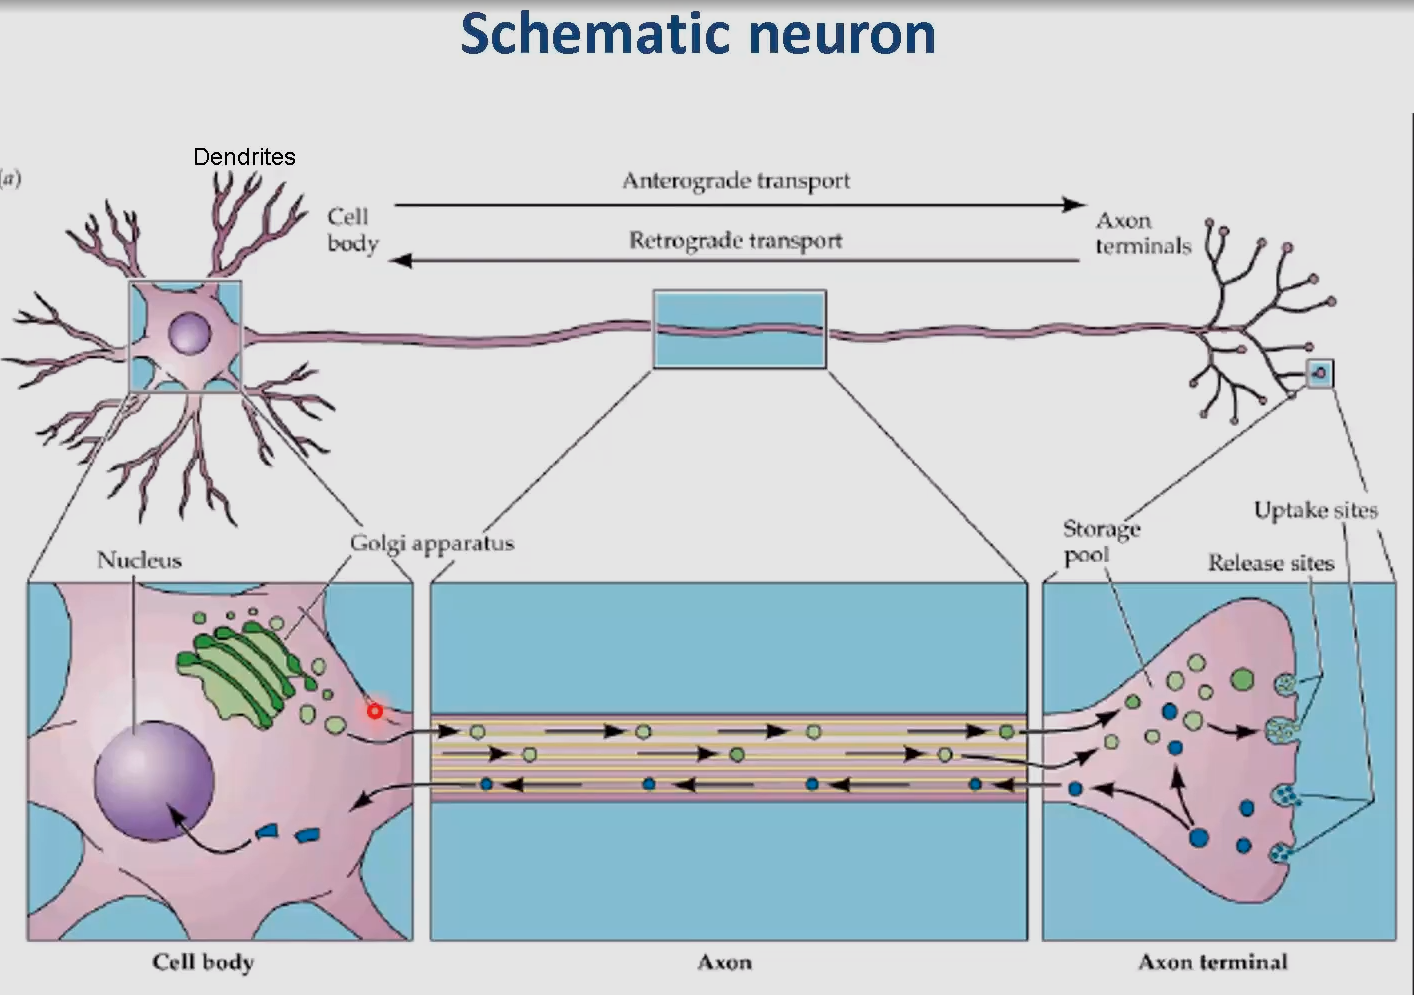
\includegraphics[width=0.5\textwidth]{assets/schematic-neuron.png}
    \caption{Schematic neuron}
    \end{figure}
    
    \begin{figure}[H]
    \centering
    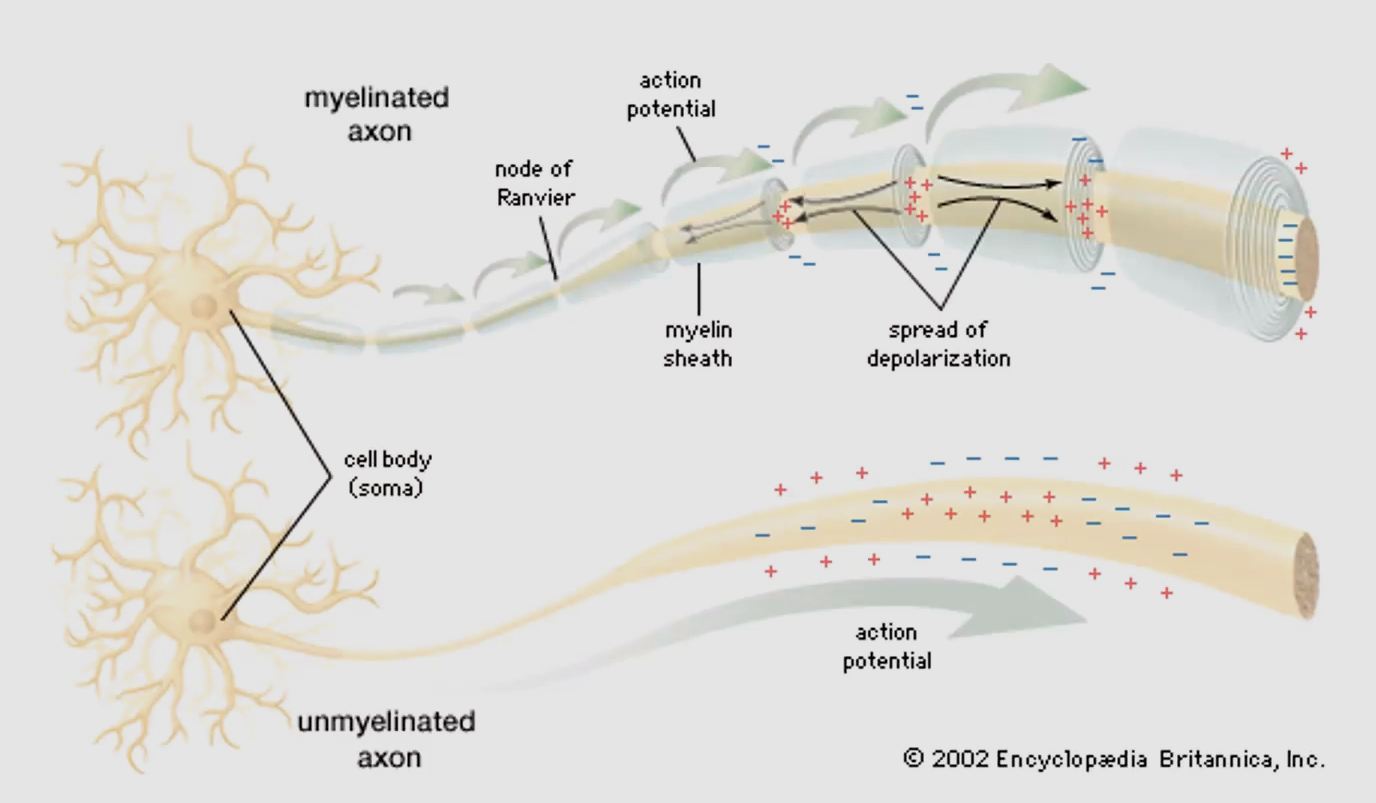
\includegraphics[width=0.5\textwidth]{assets/axon.png}
    \caption{Axon}
    \end{figure}
    
    \begin{figure}[H]
    \centering
    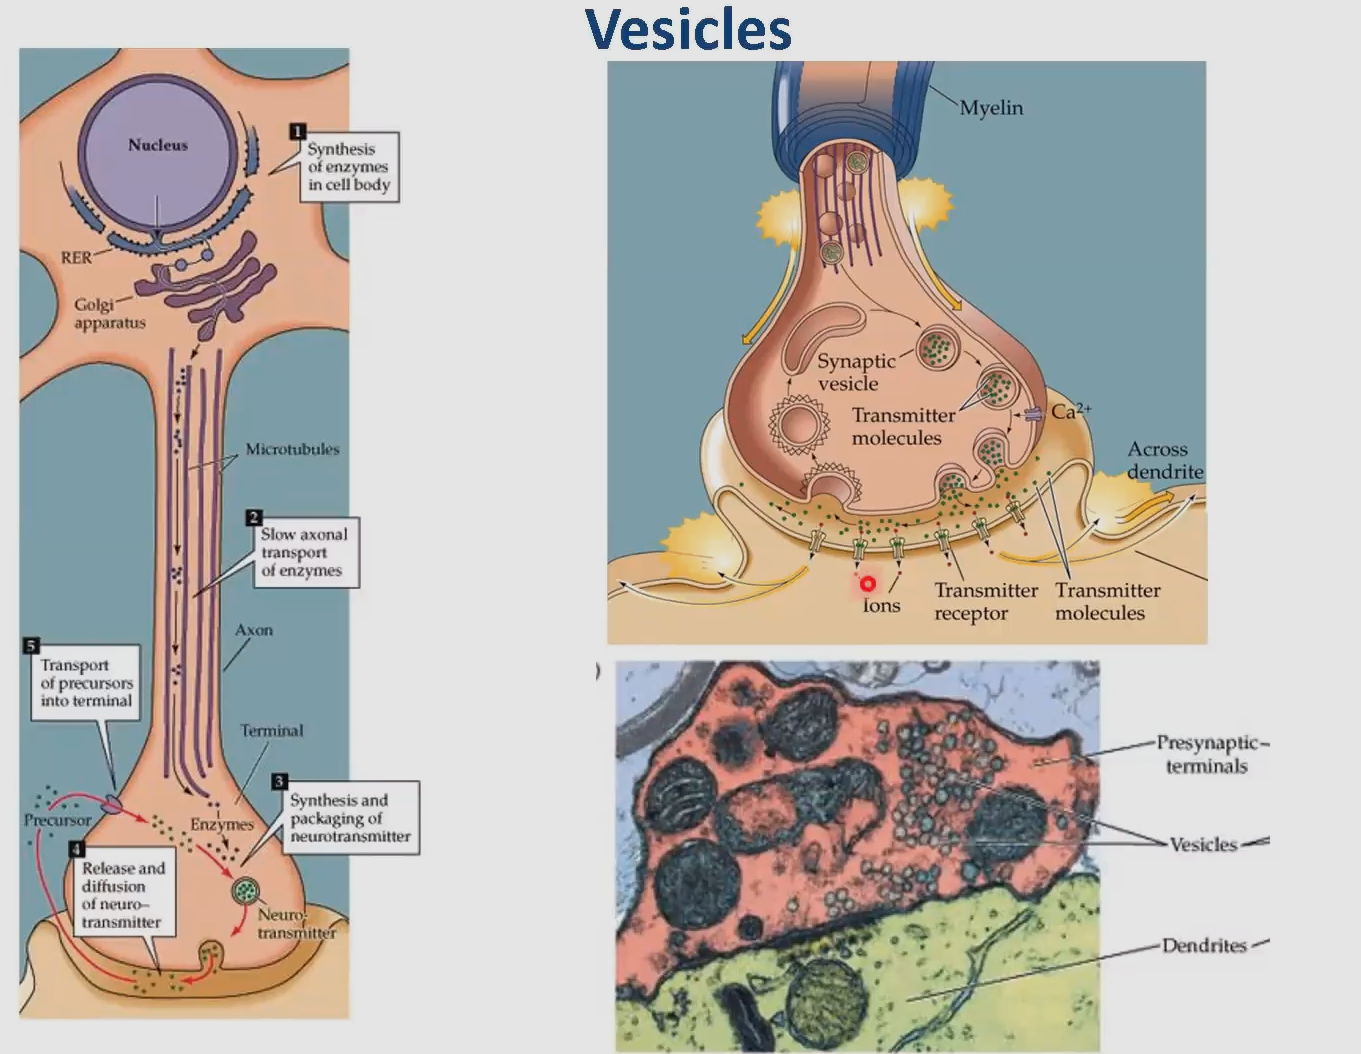
\includegraphics[width=0.5\textwidth]{assets/vesicles.png}
    \caption{Vesicles}
    \end{figure}
    
    \subsubsection{Sequence of events}
    
    \begin{enumerate}
        \item Neurotransmitter release
        \item Receptor binding
        \item Ion channels open or close
        \item Conductance change causes current flow
        \item Postsynaptic potential changes
        \item Postsynaptic cells
        \item Summation determines whether not an action potential occurs
    \end{enumerate}
    
    \subsubsection{Gross Anatomy}
    
    \begin{figure}[H]
    \centering
    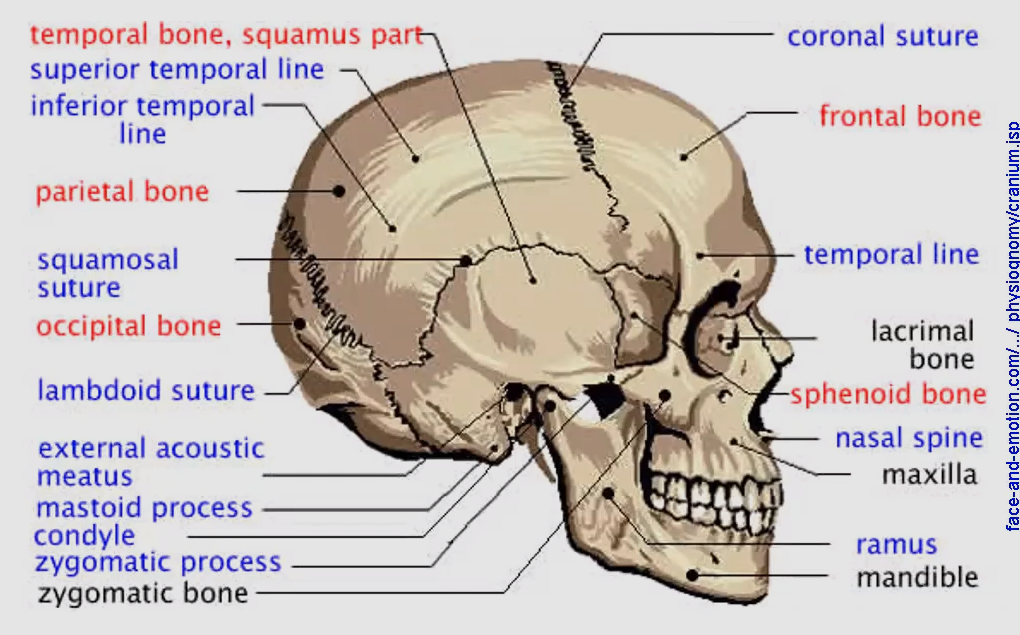
\includegraphics[width=0.5\textwidth]{assets/gross-anatomy.png}
    \caption{Gross anatomy}
    \end{figure}
    
    \begin{figure}[H]
    \centering
    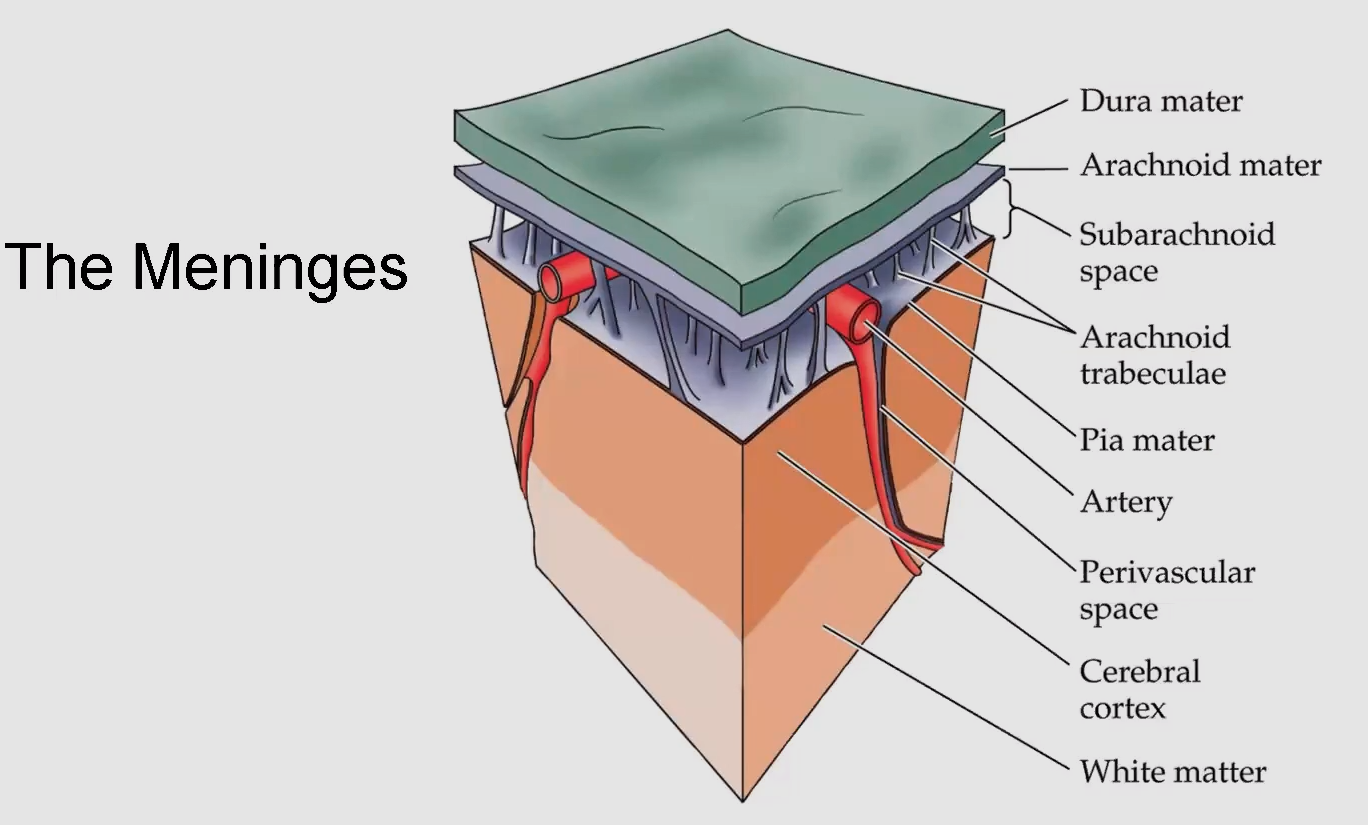
\includegraphics[width=0.5\textwidth]{assets/gross-anatomy-2.png}
    \caption{Gross anatomy 2}
    \end{figure}
    
    \begin{figure}[H]
    \centering
    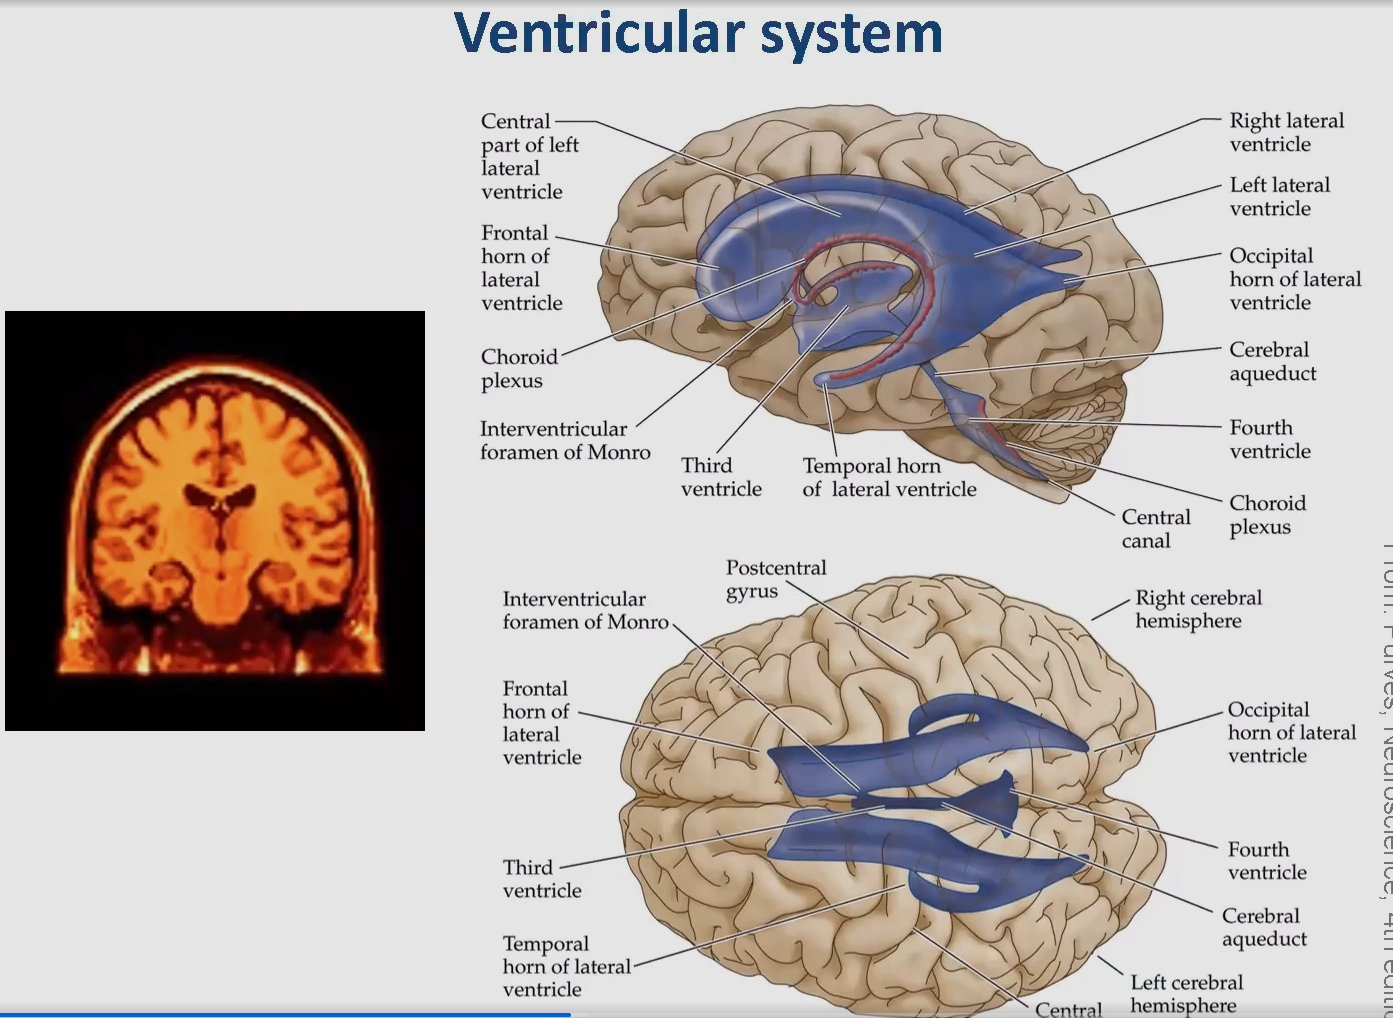
\includegraphics[width=0.5\textwidth]{assets/ventricular-system.png}
    \caption{Ventricular system}
    \end{figure}
    
    \subsubsection{Directions of Orientation in the CNS:}
    
    \begin{itemize}
        \item Anterior: Toward the front.
        \item Posterior: Toward the back.
        \item Inferior: Toward the bottom.
        \item Superior: Toward the top of the head/body.
        \item Medial: Toward the middle/midline.
        \item Lateral: Away from the middle/midline.
        \item Rostral: Toward the nose.
        \item Caudal: Toward the tail/rear.
        \item Proximal: Near the trunk/center.
        \item Distal: Away from the center.
        \item Dorsal: Toward the back.
        \item Ventral: Toward the belly.
        \item Ipsilateral: On the same side.
        \item Contralateral: On the opposite side.
        \item Bilateral: On both sides.
        \item Unilateral: On one side.
    \end{itemize}
    
    \begin{figure}[H]
    \centering
    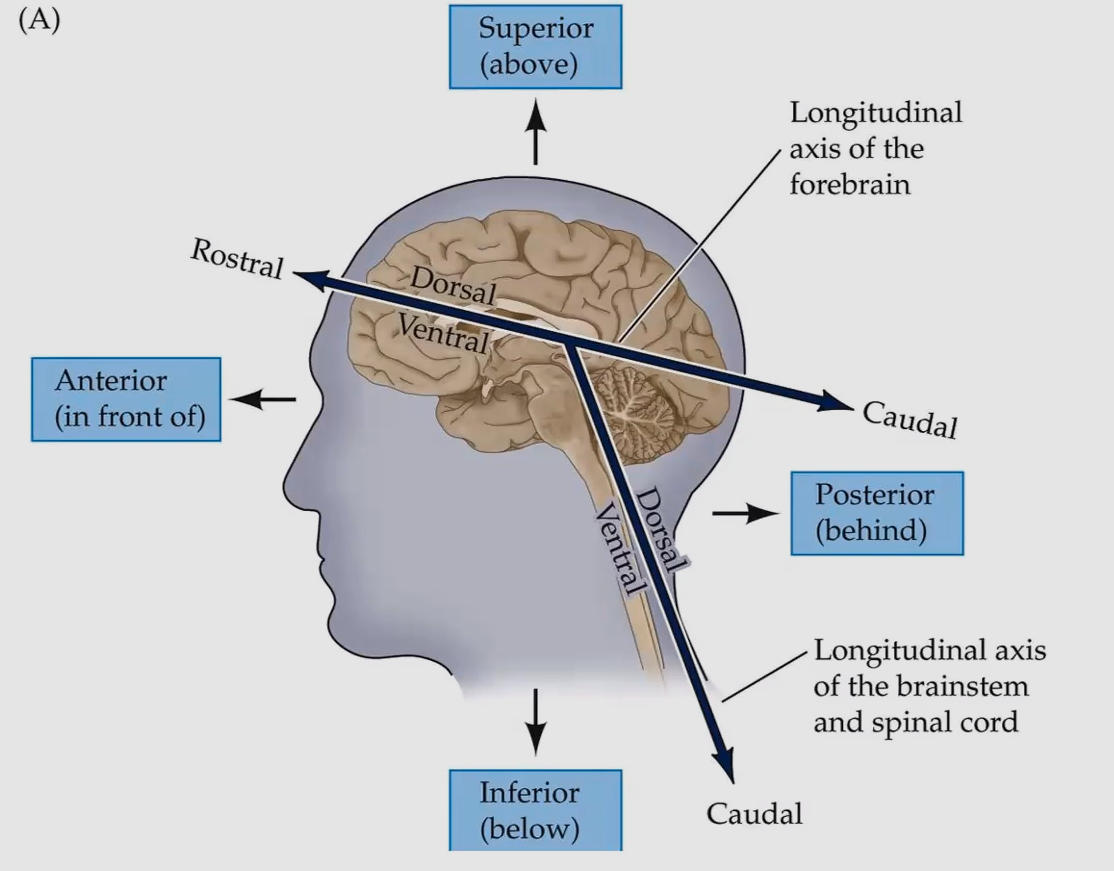
\includegraphics[width=0.5\textwidth]{assets/central-nervous-system.png}
    \caption{Central nervous system}
    \end{figure}
    
    \begin{figure}[H]
    \centering
    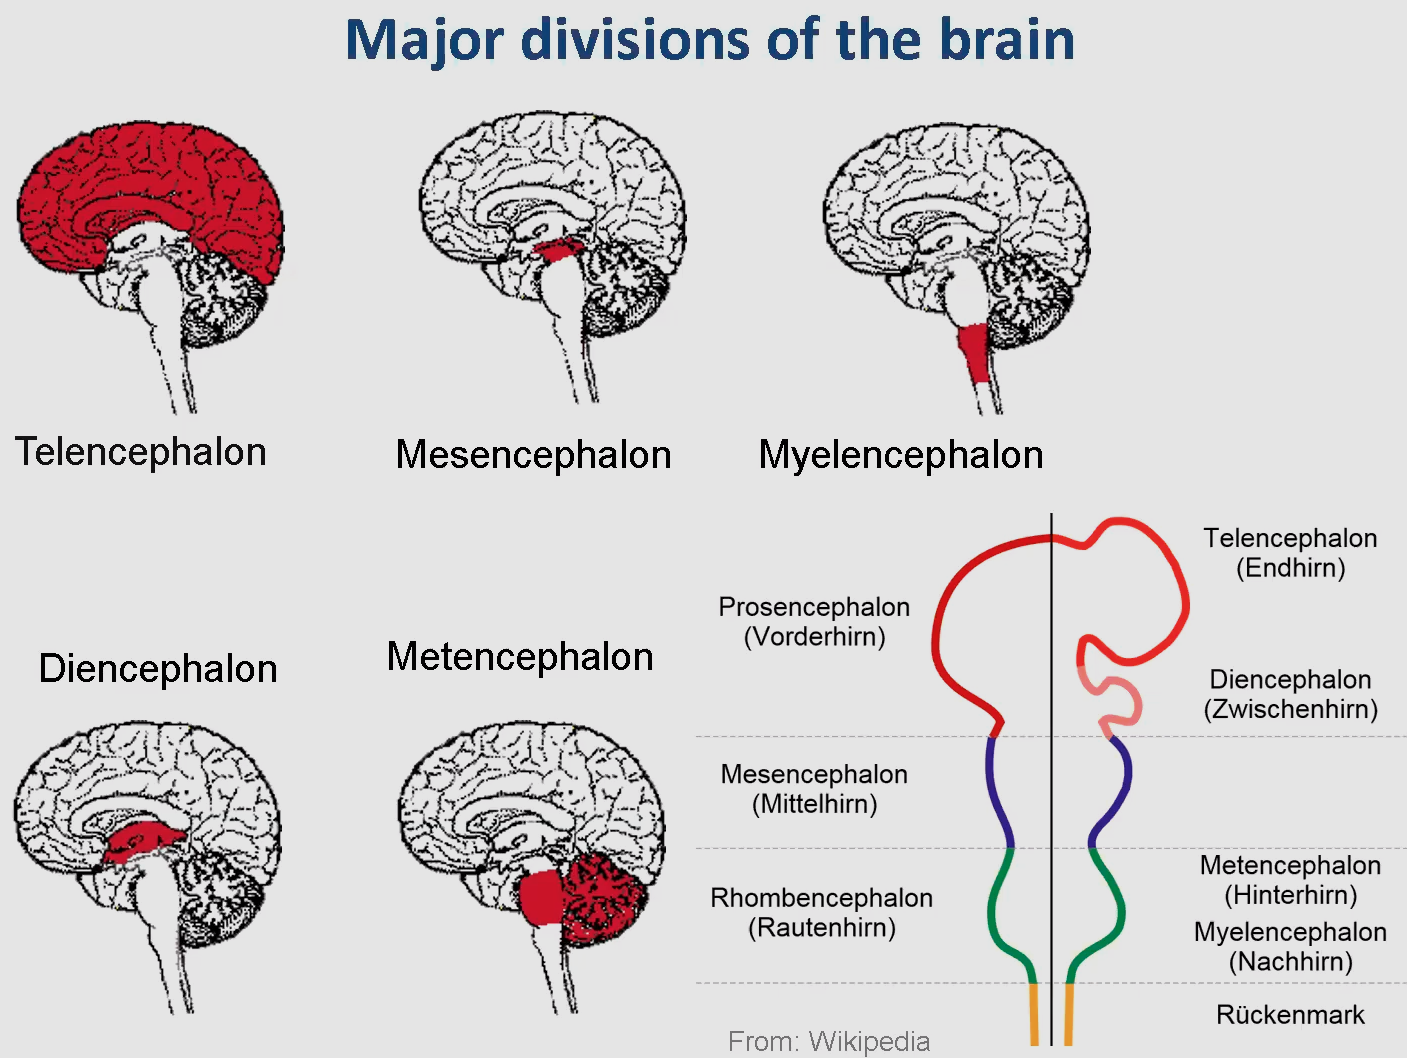
\includegraphics[width=0.5\textwidth]{assets/division-brain.png}
    \caption{Brain division}
    \end{figure}
    
    \subsubsection{Hypothalamus}
    
    \noindent \textbf{Upper Brain Stem: Diencephalon}
    
    \begin{itemize}
        \item Hypothalamus
          \begin{itemize}
            \item Structure
              \begin{itemize}
                \item Very small
                \item Contains an important collection of nuclei
              \end{itemize}
            \item Function
              \begin{itemize}
                \item Controls autonomic mechanisms
                \item Link to endocrine system
              \end{itemize}
          \end{itemize}
    \end{itemize}
    
    \subsubsection{Limbic System}
    
    \begin{itemize}
        \item Structure
          \begin{itemize}
            \item Structures on medial and basal surfaces of cerebral hemispheres
            \item Cingulate gyrus + parahippocampal gyrus + ...
            \item Anatomic circuits include basolateral circuit and the Papez circuit
          \end{itemize}
        \item Function
          \begin{itemize}
            \item Emotional expression
            \item Memory acquisition
            \item Fear conditioning
            \item Violence and aggression
          \end{itemize}
    \end{itemize}
    
    \subsubsection{Basal Ganglia}
    
    \begin{itemize}
        \item Structure
          \begin{itemize}
            \item Collection of nuclei embedded deep within cortex
            \item Partially surround the thalamus
            \item Sensory projections to cerebrum
            \item Efferents to other nervous system structures
          \end{itemize}
        \item Function
          \begin{itemize}
            \item Regulate voluntary movement
            \item Integrative or just a relay station?
          \end{itemize}
        \item Pathology
          \begin{itemize}
            \item Movement disorders (Parkinson's)
          \end{itemize}
    \end{itemize}

\subsubsection{The Human Brain}
\begin{itemize}
    \item The average human brain weighs about 1.5 kg and has a volume of approximately 1.1-1.2 liters.
    \item Despite the similarities in neuron cells across species, human brains have unique characteristics in terms of size and complexity.
\end{itemize}

\subsubsection{Brain Functions}
The brain's primary functions include:
\begin{itemize}
    \item Encoding and decoding stimuli from the environment.
    \item Integrating sensory information to form perceptions.
    \item Making decisions and executing movements, which collectively define our behavior.
\end{itemize}

\subsection{Comparison between Brains and Computers}
Understanding the similarities and differences between brains and computers is crucial in neuroinformatics:
\begin{itemize}
    \item Similarities include processing information, performing logical operations, memory storage, use of electrical signaling, learning capabilities, and energy consumption.
    \item Differences involve aspects such as massive parallelism, separation of memory and processing, adaptability, chemical signaling, analog computation, and energy efficiency.
\end{itemize}

\subsection{Neuromorphic Engineering}
A significant part of neuroinformatics is understanding and creating neuromorphic systems:
\begin{itemize}
    \item Neuromorphic chips like IBM's TrueNorth and Intel's Loihi are designed to mimic the brain's neural architecture.
    \item These chips are characterized by their parallel processing capabilities and energy efficiency, making them suitable for various applications in computing and robotics.
\end{itemize}

\subsection{Organization of the Brain}
\subsubsection{Gross Anatomy of the Brain}
\begin{itemize}
    \item The brain is divided into several major parts: the cerebrum, cerebellum, and brainstem.
    \item The cerebrum, the largest part, is responsible for higher brain functions like thought and action.
    \item The cerebellum, located under the cerebrum, plays a role in coordination and balance.
    \item The brainstem connects the brain to the spinal cord and controls basic life functions like breathing and heartbeat.
\end{itemize}

\subsubsection{Ventricular System}
\begin{itemize}
    \item Consists of four interconnected cavities (ventricles) in the brain filled with cerebrospinal fluid (CSF).
    \item CSF cushions the brain, removes waste products, and provides a stable chemical environment.
\end{itemize}
The ventricular system is an essential component of the human brain, responsible for the production and circulation of cerebrospinal fluid (CSF). This fluid plays a critical role in maintaining brain health and function. In this article, we will explore the structure and functions of the ventricular system in detail.

The ventricular system consists of a series of interconnected cavities known as ventricles. These ventricles are numbered and include:

\begin{enumerate}
  \item The \textbf{Lateral Ventricles} (First and Second Ventricles): These are located in the cerebral hemispheres and are the largest of the ventricles.
  \item The \textbf{Third Ventricle}: This is a narrow, slit-like cavity located at the midline of the brain.
  \item The \textbf{Cerebral Aqueduct} (Aqueduct of Sylvius): This is a narrow canal connecting the third ventricle to the fourth ventricle.
  \item The \textbf{Fourth Ventricle}: This is located in the hindbrain and connects to the central canal of the spinal cord.
\end{enumerate}

The walls of these ventricles are lined with ependymal cells, which are specialized cells responsible for producing CSF.
\paragraph{Functions of the Ventricular System}

The ventricular system serves several important functions, including:

\begin{itemize}
  \item \textbf{Production of Cerebrospinal Fluid (CSF)}: The ependymal cells lining the ventricles produce CSF, a clear and colorless fluid that bathes the brain and spinal cord, providing mechanical support and cushioning.
  \item \textbf{Circulation of CSF}: CSF is circulated throughout the brain and spinal cord, delivering essential nutrients and removing waste products.
  \item \textbf{Protection}: CSF acts as a shock absorber, protecting the brain from mechanical injuries.
  \item \textbf{Transportation}: It facilitates the transportation of hormones and other substances within the central nervous system.
\end{itemize}

\subsubsection{Central and Peripheral Nervous Systems}
\begin{itemize}
    \item The CNS is the control center for the body, processing and responding to sensory information.
    \item The PNS consists of nerves and ganglia outside the CNS, transmitting signals to and from different body parts.
\end{itemize}

\subsection{The Limbic System}
\begin{itemize}
    \item The limbic system is a complex set of structures located on both sides of the thalamus, just beneath the cerebrum.
    \item It supports a variety of functions, including emotion, behavior, motivation, long-term memory, and olfaction.
\end{itemize}

The limbic system is not a single, distinct structure but rather a collection of interconnected regions in the brain. Key components of the limbic system include:

\paragraph{Amygdala}

\begin{itemize}
  \item The amygdala is involved in the processing of emotions, particularly fear and aggression.
  \item It plays a vital role in the formation of emotional memories and the recognition of emotional cues in others.
\end{itemize}

\paragraph{Hippocampus}

\begin{itemize}
  \item The hippocampus is crucial for the formation and consolidation of new memories, particularly declarative and spatial memories.
  \item It plays a role in spatial navigation and cognitive mapping.
\end{itemize}

\paragraph{Hypothalamus}

\begin{itemize}
  \item The hypothalamus regulates various autonomic functions, including body temperature, hunger, thirst, and sleep.
  \item It also controls the release of hormones from the pituitary gland, which influence the endocrine system.
\end{itemize}

\paragraph{Thalamus}

\begin{itemize}
  \item The thalamus acts as a relay station for sensory information, directing it to the appropriate areas of the cortex for further processing.
  \item It plays a role in consciousness and awareness.
\end{itemize}

\subsubsection{Functions of the Limbic System}

The limbic system serves several critical functions, including:

\begin{itemize}
  \item \textbf{Emotion Processing}: The limbic system processes and regulates emotions, such as fear, pleasure, and anger.
  \item \textbf{Memory Formation}: It plays a central role in the formation and consolidation of memories, particularly emotional and declarative memories.
  \item \textbf{Homeostasis}: The limbic system helps maintain physiological balance by regulating basic survival instincts like hunger, thirst, and body temperature.
  \item \textbf{Reward System}: It is involved in the brain's reward pathway, which reinforces behaviors related to pleasure and survival.
\end{itemize}

\subsection{Key Brain Areas}
\begin{itemize}
    \item The thalamus acts as the brain's relay center, channeling sensory signals to the appropriate part of the cortex.
    \item The hypothalamus regulates various functions like temperature, hunger, thirst, and emotional activity.
    \item Basal ganglia are a group of structures involved in controlling voluntary motor movements, procedural learning, routine behaviors, and emotions.
\end{itemize}

\subsection{Lobes of the Cerebral Cortex}
\begin{itemize}
    \item The cerebral cortex is divided into four lobes: frontal, parietal, temporal, and occipital.
    \item Each lobe is associated with different functions: 
        \begin{itemize}
            \item Frontal Lobe: involved in decision making, problem solving, planning, and parts of speech and movement.
            \item Parietal Lobe: processes sensory information such as temperature, taste, touch, and movement.
            \item Temporal Lobe: involved in memory, emotion, hearing, and language.
            \item Occipital Lobe: primarily responsible for vision.
        \end{itemize}
\end{itemize}

\subsection{Cytoarchitecture and Brodmann's Areas}
\begin{itemize}
    \item Cytoarchitecture refers to the study of cellular composition of the brain's structures.
    \item Brodmann’s areas are based on the types of neurons and their organization and are used to distinguish between different functional areas of the brain.
    \item This classification aids in understanding the diverse functions the brain performs and how different regions interact.
\end{itemize}

\subsection{Soup vs Spark}

\begin{itemize}
    \item is synaptic transmission mediated chemically or by direct electrical transfer of charge
    \item NMJ accepted that it was chemical $\rightarrow$ certain aspects too fast to be mediated chemically
\end{itemize}

\subsection{Frog experiment}

\begin{itemize}
    \item to support neurotransmitter hypothesis
    \item first frogs heartbeat slowed, second frog inhibitory effect of vagus transferred
    \item building connection of synapsis not rebuilding brain
\end{itemize}

\begin{figure}[H]
    \centering
    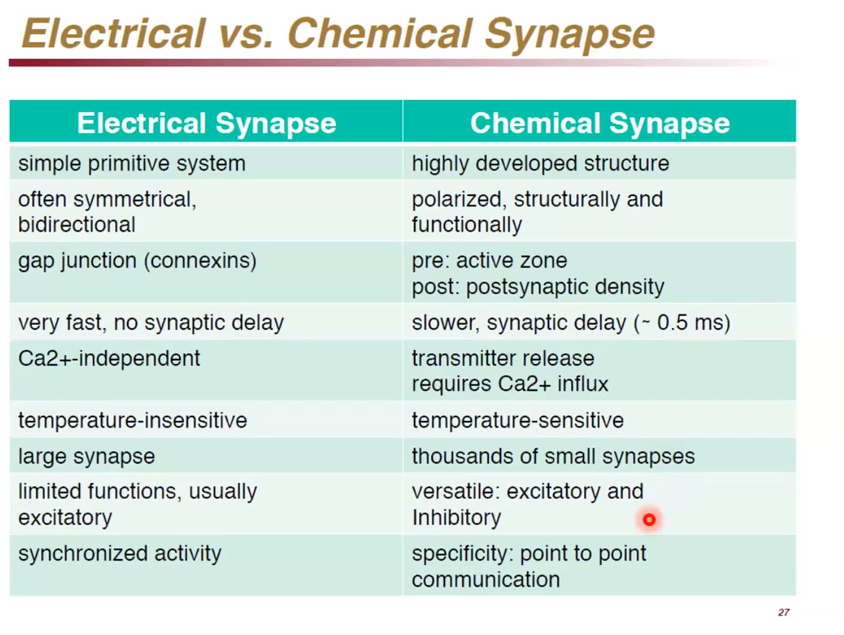
\includegraphics[width=0.5\textwidth]{assets/synapse.png}
    \caption{Synapse}
    \end{figure}
    
    \section{Brain Structure}
    
    \noindent \textbf{Telencephalon Regions}
    
    The cerebral cortex (neocortex) is anatomically divided into 4 lobes
    
    \begin{figure}[H]
    \centering
    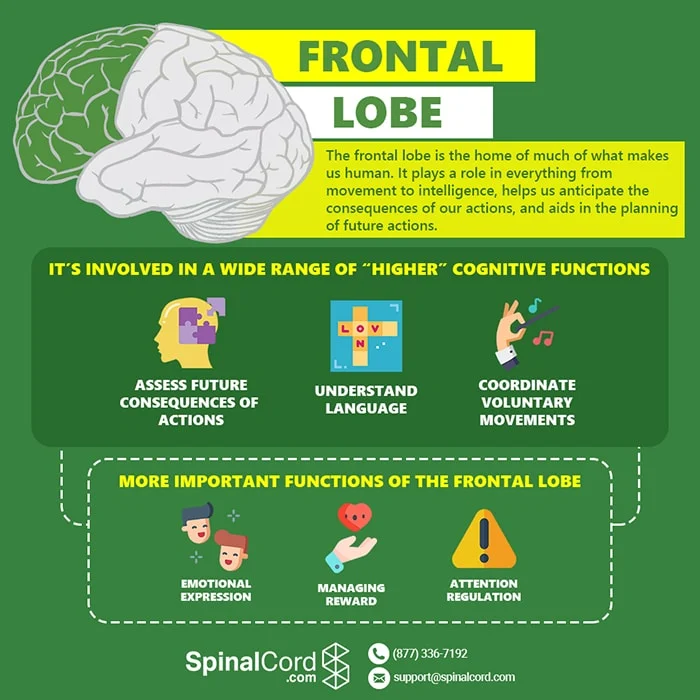
\includegraphics[width=0.5\textwidth]{assets/frontalLobe.png}
    \caption{Frontal lobe}
    \end{figure}
    
    \begin{figure}[H]
    \centering
    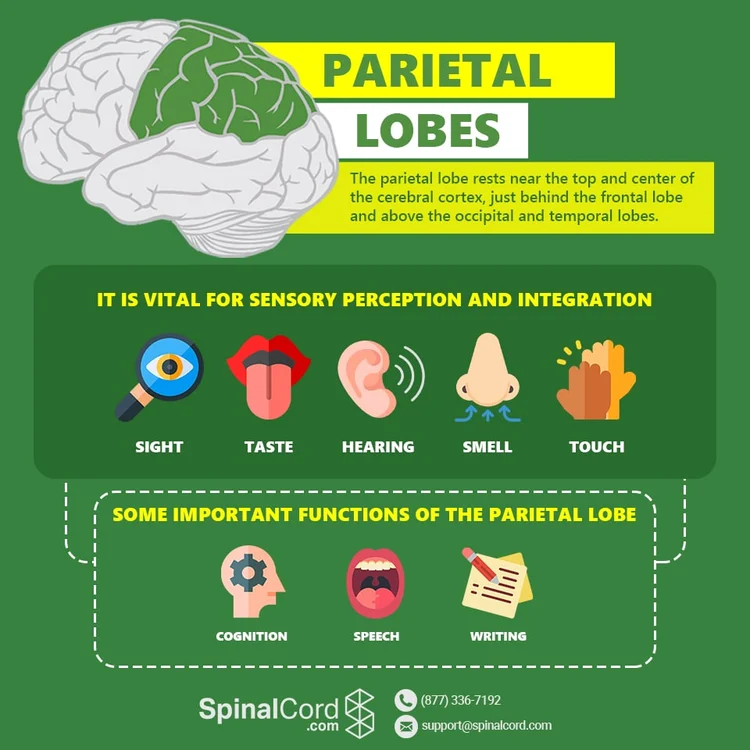
\includegraphics[width=0.5\textwidth]{assets/parietalLobe.png}
    \caption{Parietal lobe}
    \end{figure}
    
    \noindent separated from the frontal lobe by the \textbf{central sulcus}. Primary lobe for somatosensory processing (afferent inputs from receptors in the skin). Additionally, subserves other sensori-motor functions.
    
    \begin{figure}[H]
    \centering
    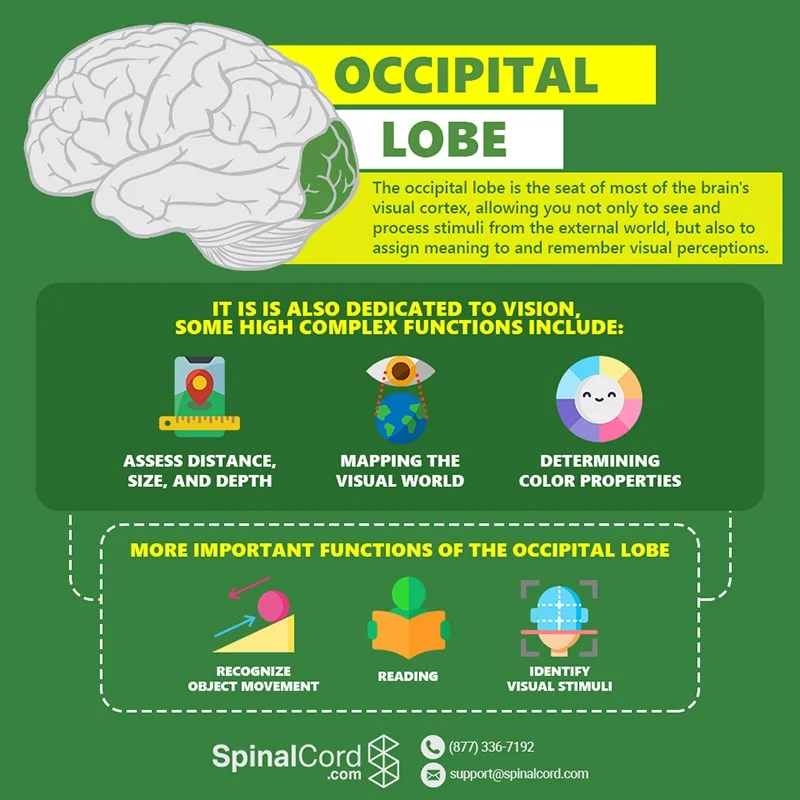
\includegraphics[width=0.5\textwidth]{assets/occipitalLobe.png}
    \caption{Occipital lobe}
    \end{figure}
    
    \begin{figure}[H]
    \centering
    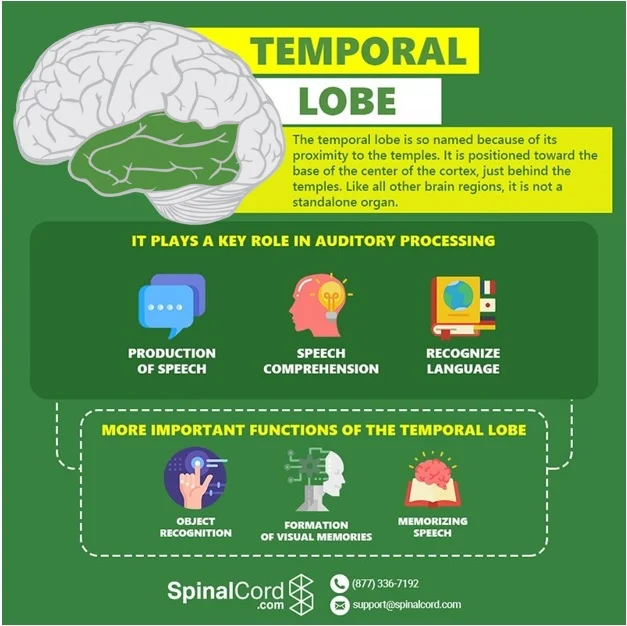
\includegraphics[width=0.5\textwidth]{assets/temporalLobe.png}
    \caption{Temporal lobe}
    \end{figure}
    
    \noindent separated from the frontal and parietal lobe by the \textbf{lateral fissure (Sylvian fissure)}. Involved in auditory processing and language comprehension \textbf{(Wernickes area)}. Additionally, responsible for visual object recognition. The medial portion of the temporal lobe includes a \textbf{portion of the hippocampal formation which is involved in formation of new memories}
    
    \begin{figure}[H]
    \centering
    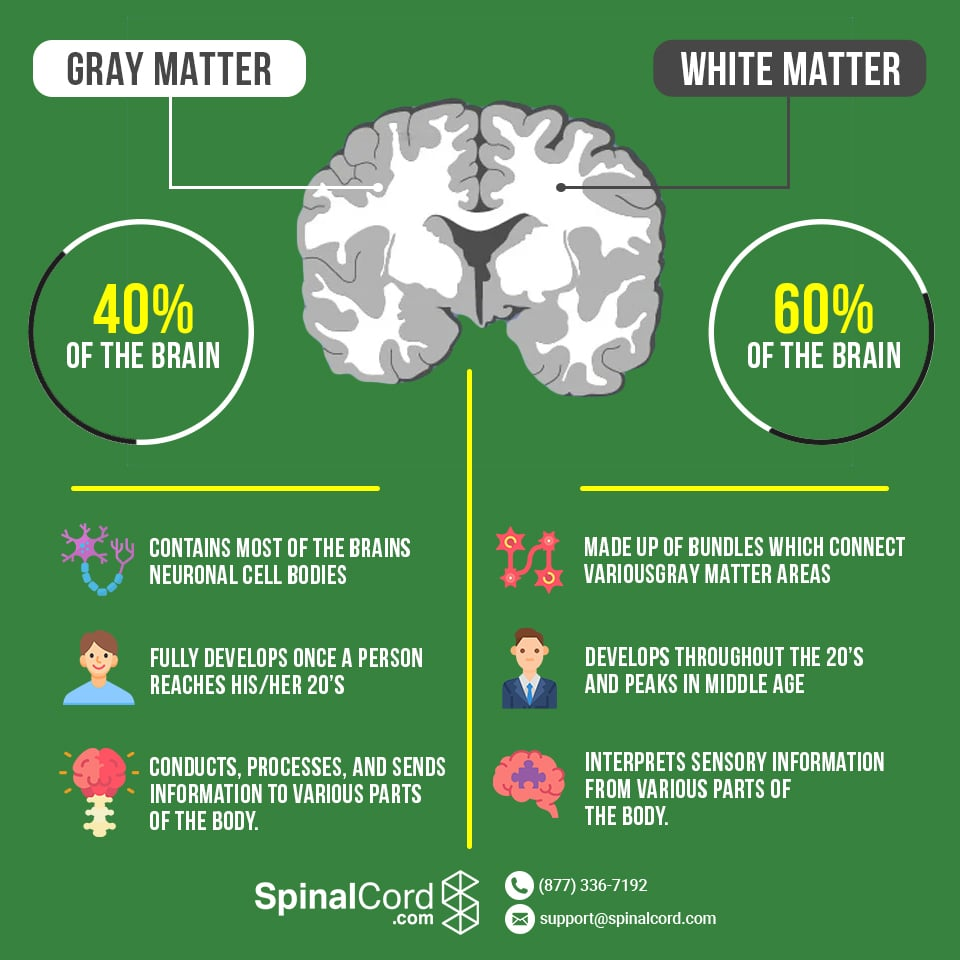
\includegraphics[width=0.5\textwidth]{assets/matter.png}
    \caption{Brain matter}
    \end{figure}
    
    \begin{figure}[H]
    \centering
    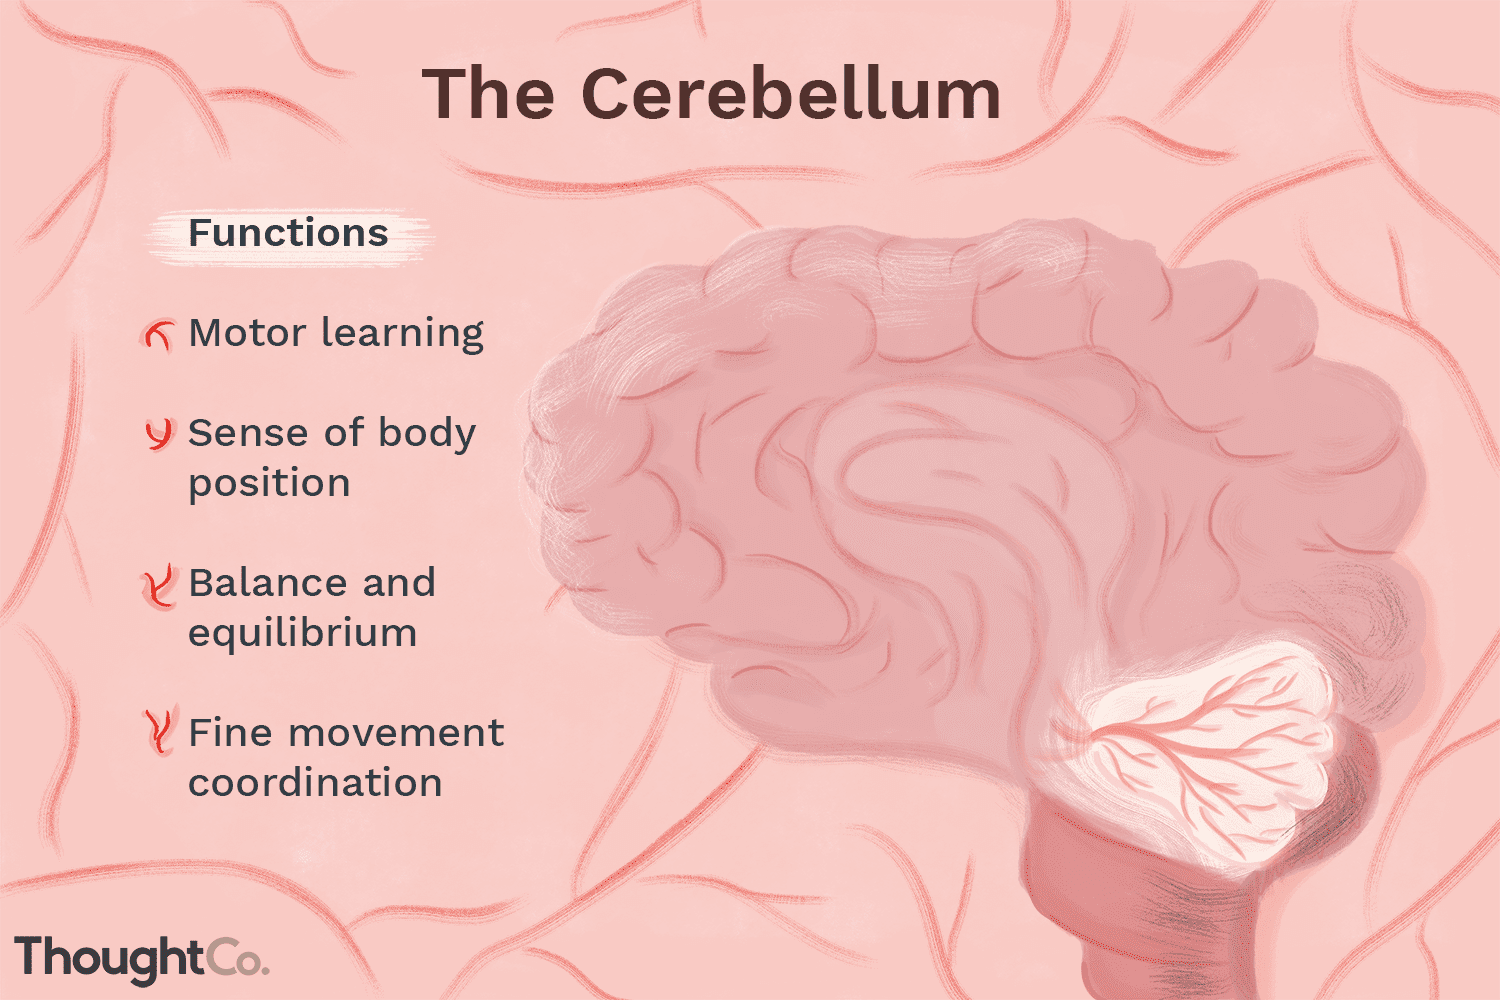
\includegraphics[width=0.5\textwidth]{assets/cerebellum.png}
    \caption{Cerebellum}
    \end{figure}
    
    \begin{figure}[H]
    \centering
    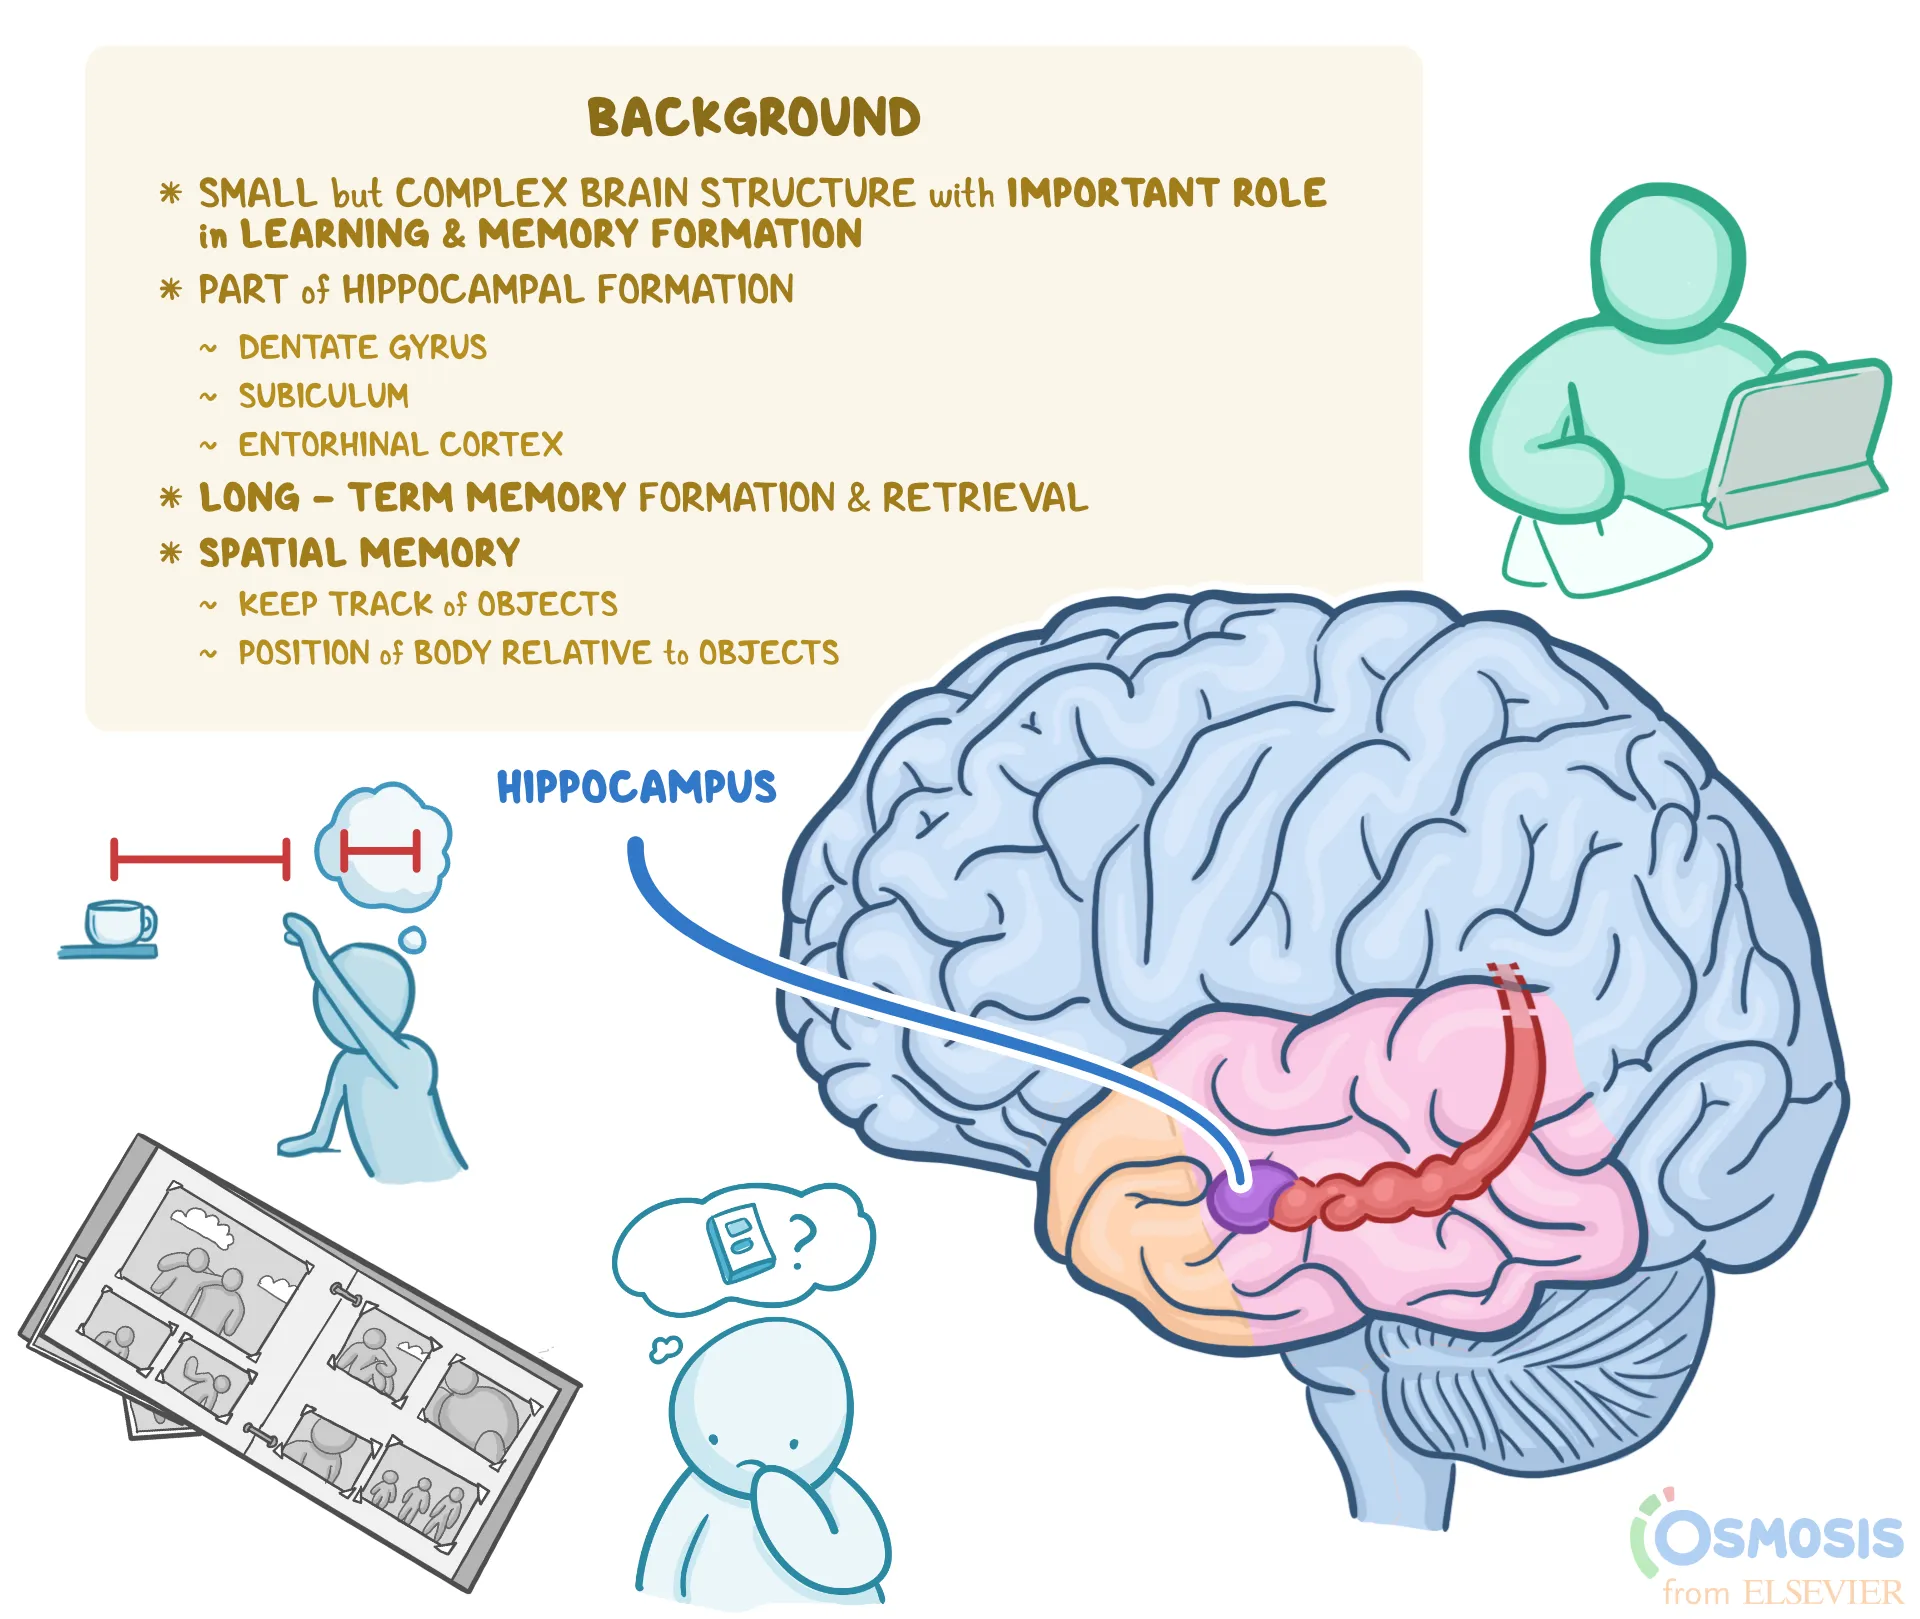
\includegraphics[width=0.5\textwidth]{assets/hippocampus.png}
    \caption{Hippocampus}
    \end{figure}
    
    \begin{figure}[H]
    \centering
    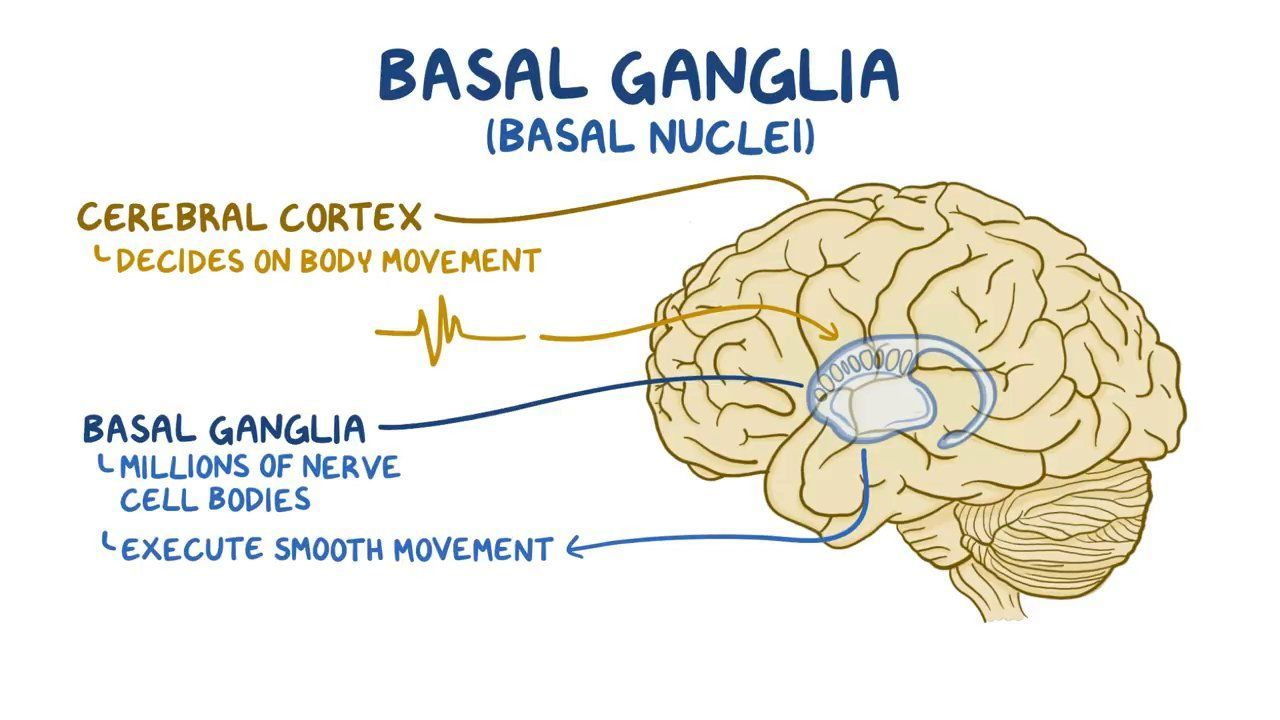
\includegraphics[width=0.5\textwidth]{assets/basalGanglia.png}
    \caption{Basal Ganglia}
    \end{figure}
    
    \noindent sub-cortical structure significantly involved in motor learning and control. Degeneration of a subset of dopaminergic neurons in the basal ganglia results in Parkinson's disease.
    
    \begin{figure}[H]
    \centering
    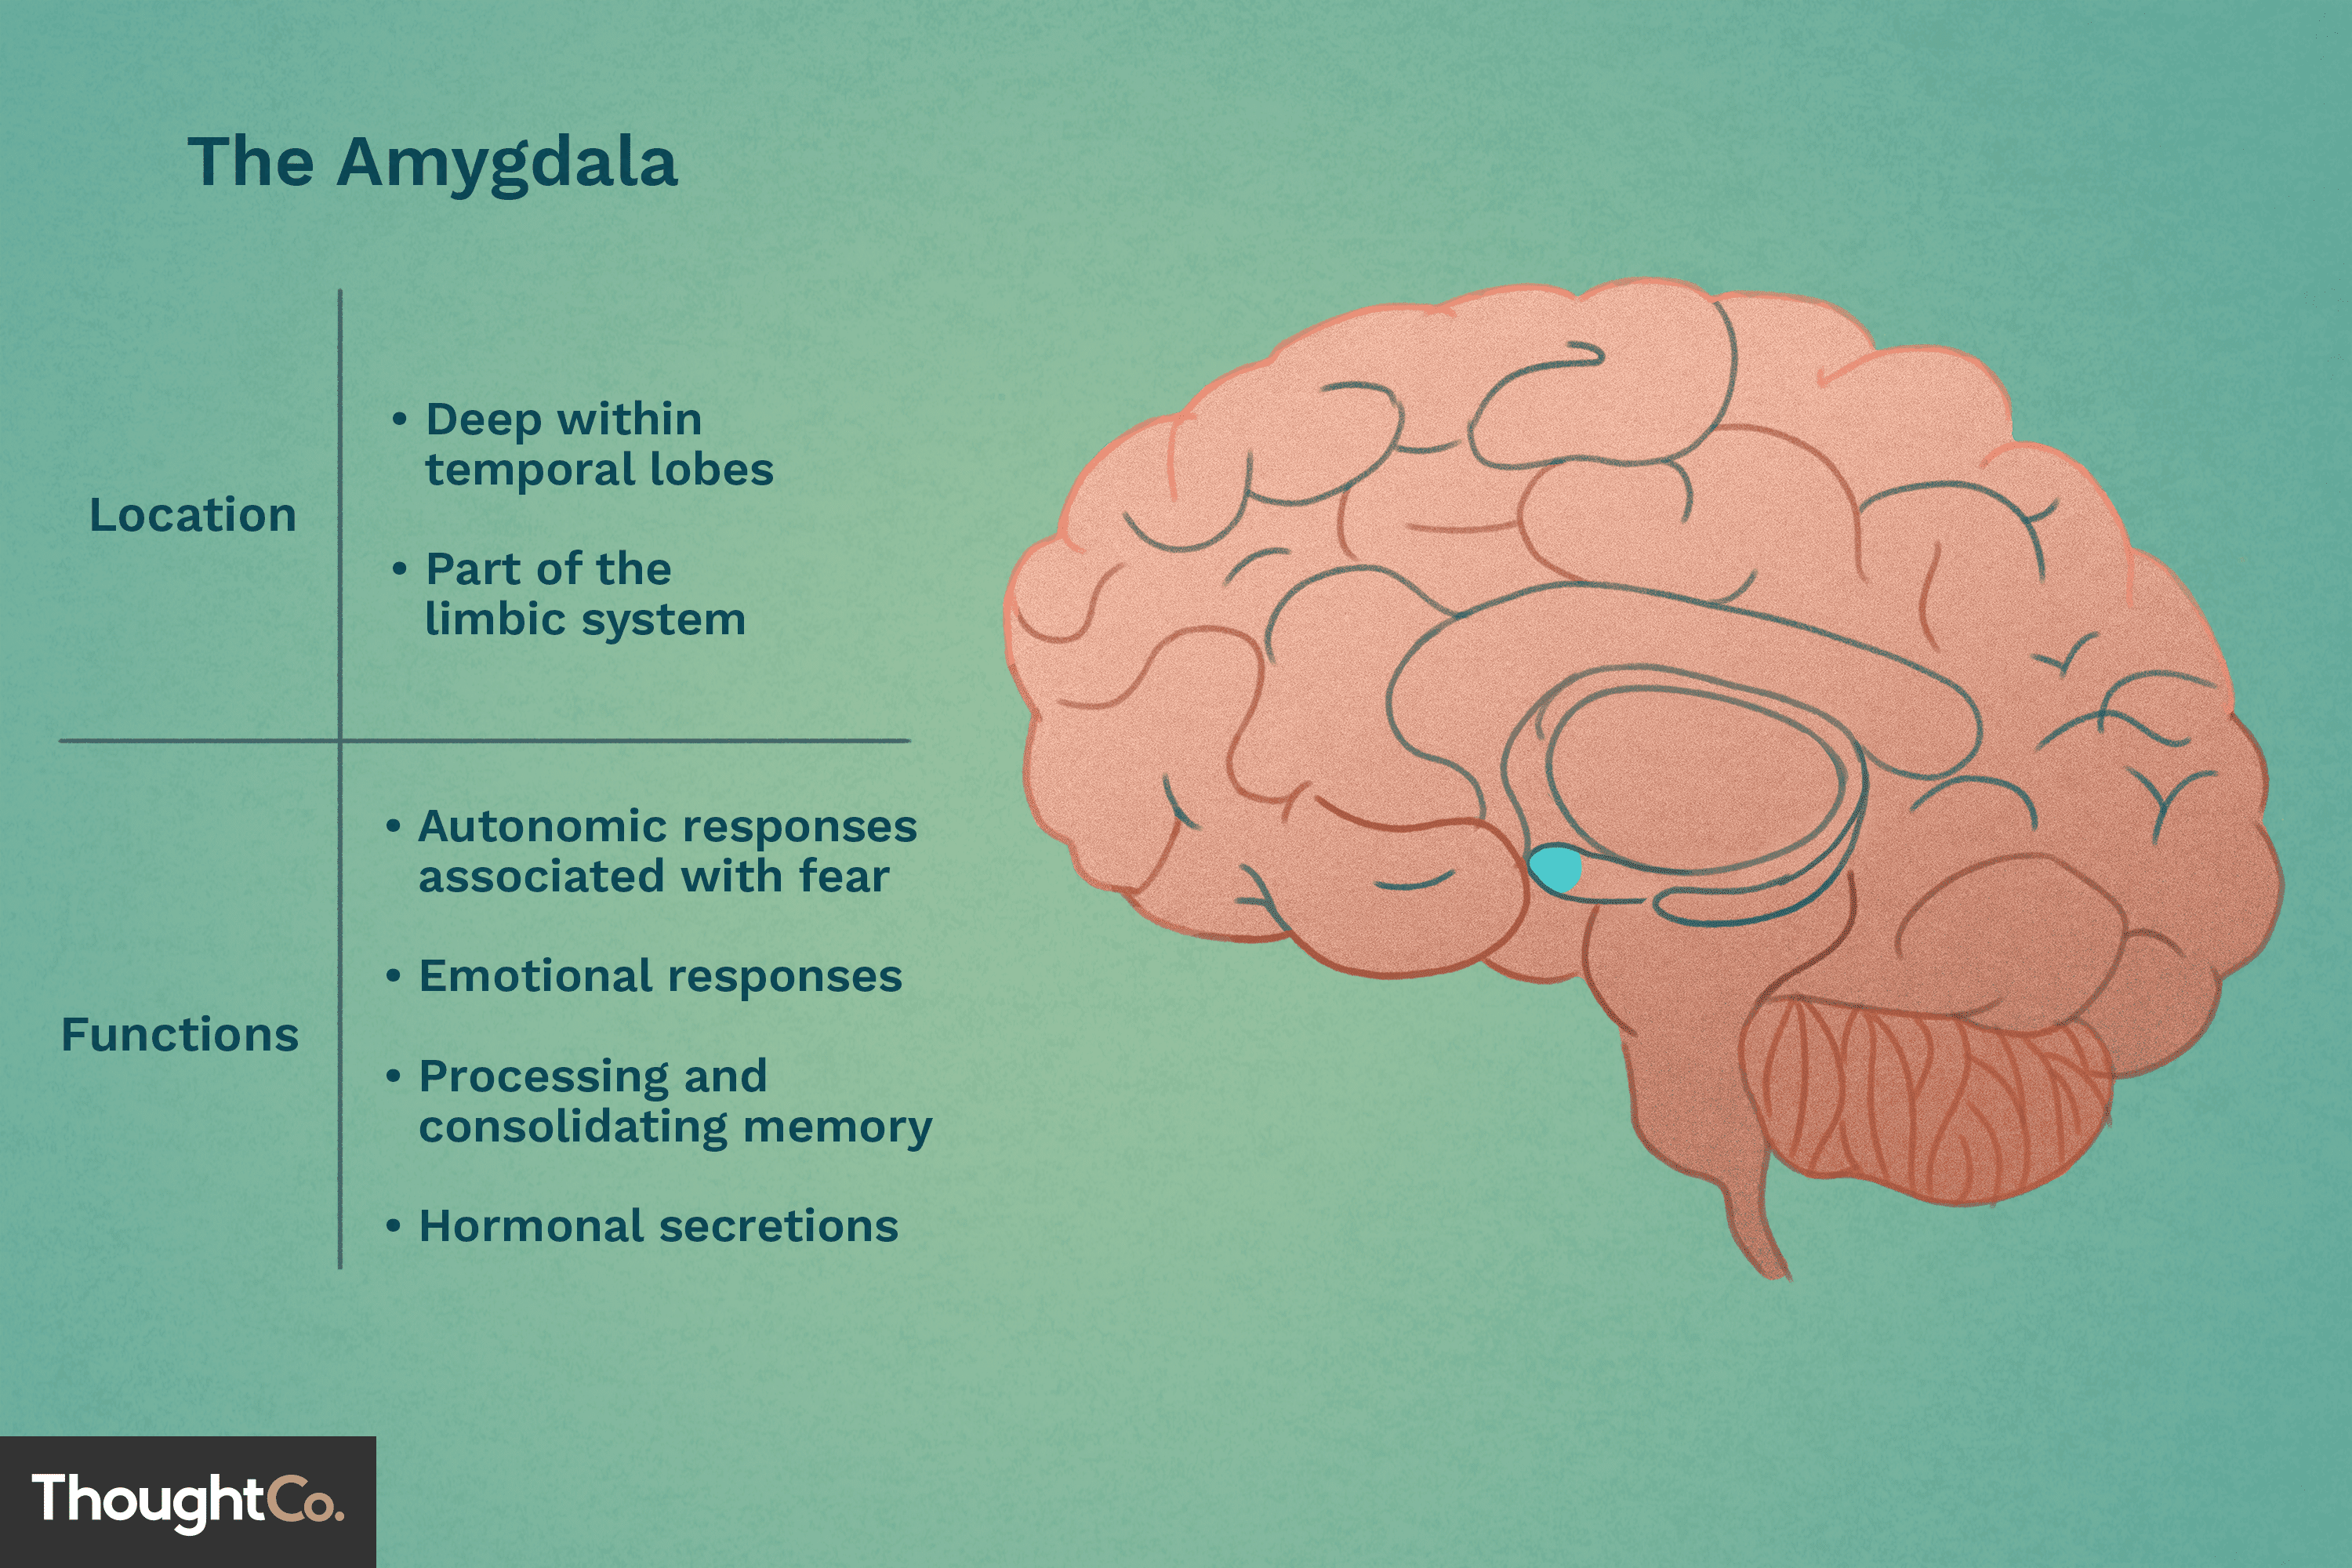
\includegraphics[width=0.5\textwidth]{assets/amygdala.png}
    \caption{Amygdala}
    \end{figure}
    
    \noindent centre for emotional processing and is strongly linked to the olfactory senses (sense of smell).
    
    \begin{figure}[H]
    \centering
    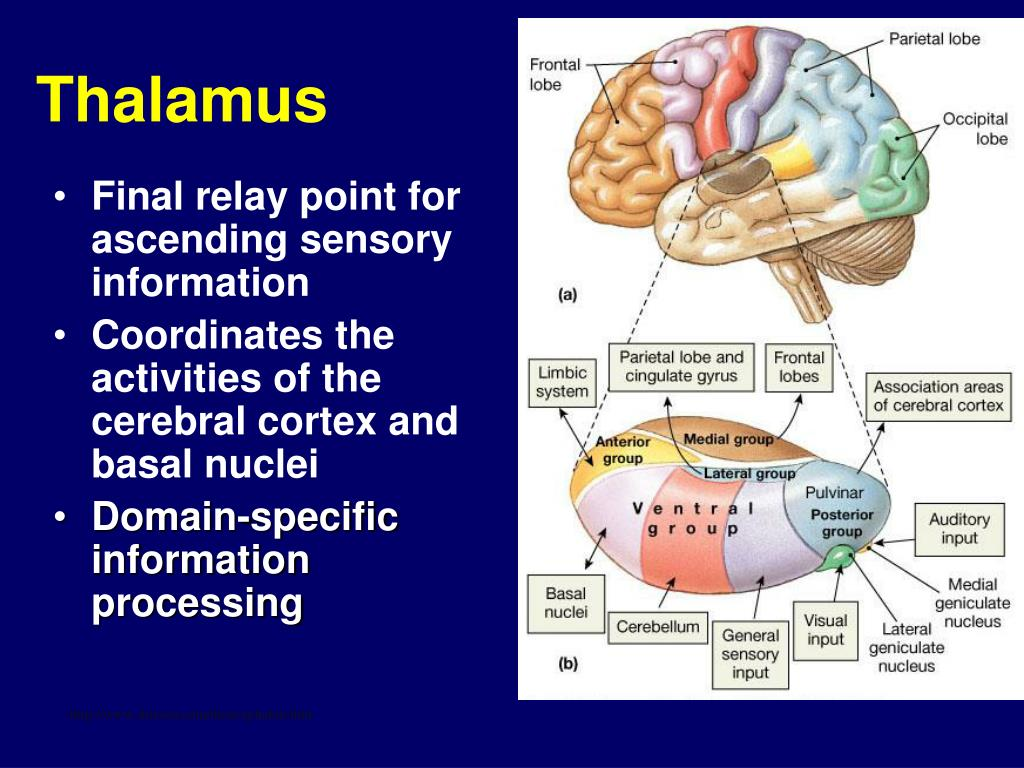
\includegraphics[width=0.5\textwidth]{assets/thalamus.png}
    \caption{Thalamus}
    \end{figure}
    
    \noindent composed of several nuclei which act as relay stations to transmit information to and from neocortex.
    
    \begin{figure}[H]
    \centering
    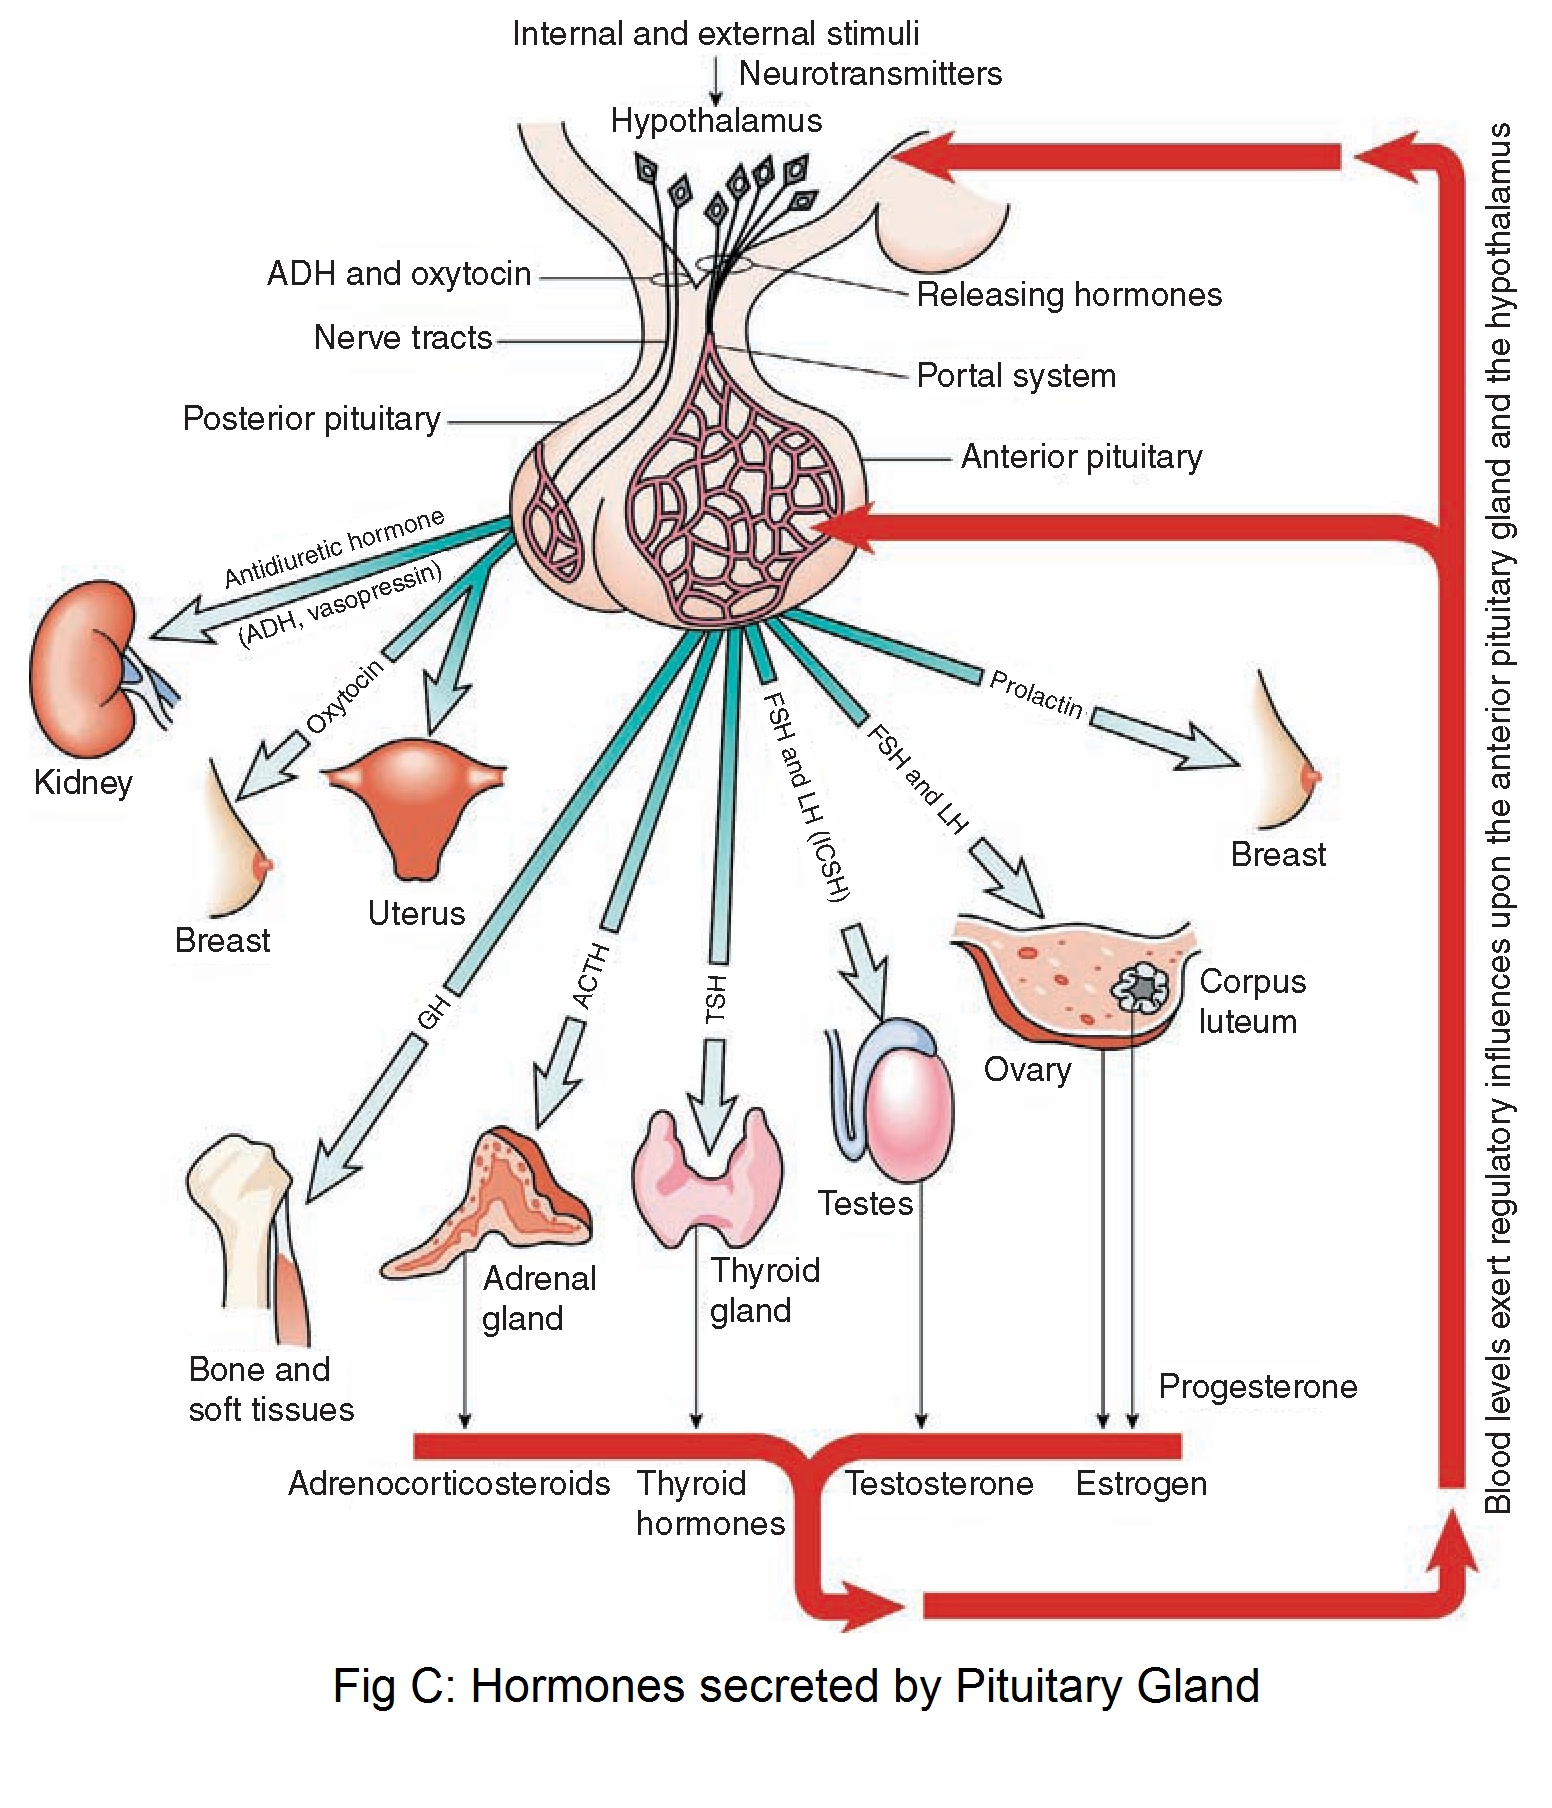
\includegraphics[width=0.5\textwidth]{assets/pituitary.png}
    \caption{Pituitary gland}
    \end{figure}
    
    \begin{figure}[H]
    \centering
    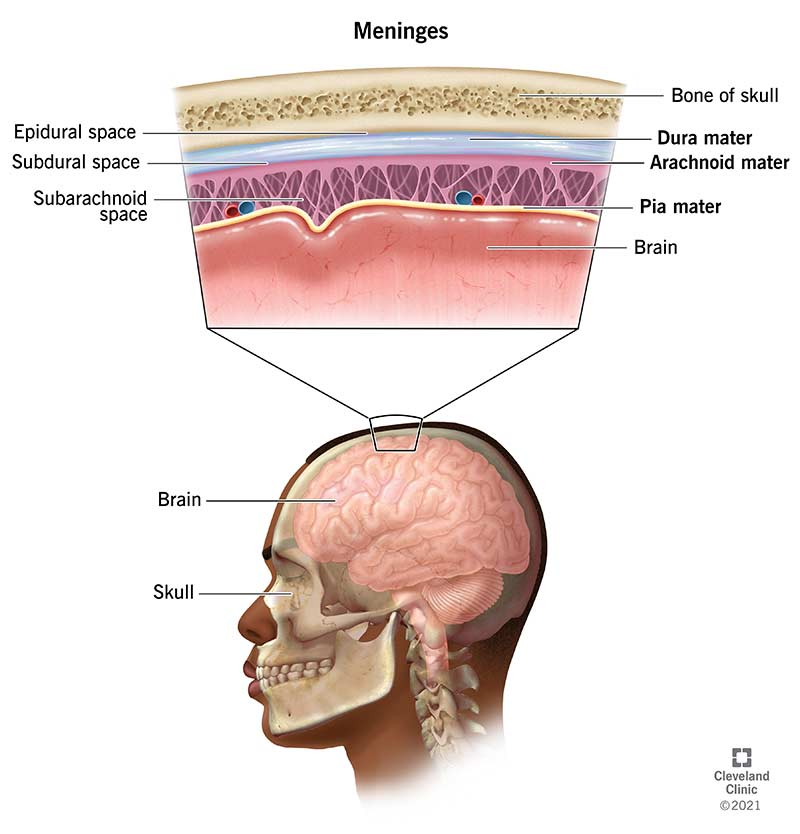
\includegraphics[width=0.5\textwidth]{assets/menings.png}
    \caption{Meninges}
    \end{figure}
    
    \noindent The brain and spinal cord are protected by three layers collectively known as meninges:
    
    \begin{itemize}
        \item dura-mater: A thick leather-like inelastic layer present directly below the bone.
        \item arachnoid-mater: A thin, delicate, middle layer present directly below the dura-mater. Has spider web like filamentous extensions into the sub-arachnoid space which reach the pia-mater
        \item pia-mater: A thin, delicate, translucent layer that directly lines the gyri/sulci of the brain, and the spinal cord. Rich in blood-vessels that supply oxygen and nutrients to the brain. Functionally, it forms the blood brain barrier (BBB).
    \end{itemize}
    
    \noindent \textbf{Diencephalon Regions}
    
    Thalamus: composed of several nuclei which act as relay stations to transmit information to and from neocortex.
    
    Hypothalamus: required for regulation of autonomic bodily functions
    
    Pituitary Gland: regulation of the endocrine (hormonal) system
    
    \begin{figure}[H]
    \centering
    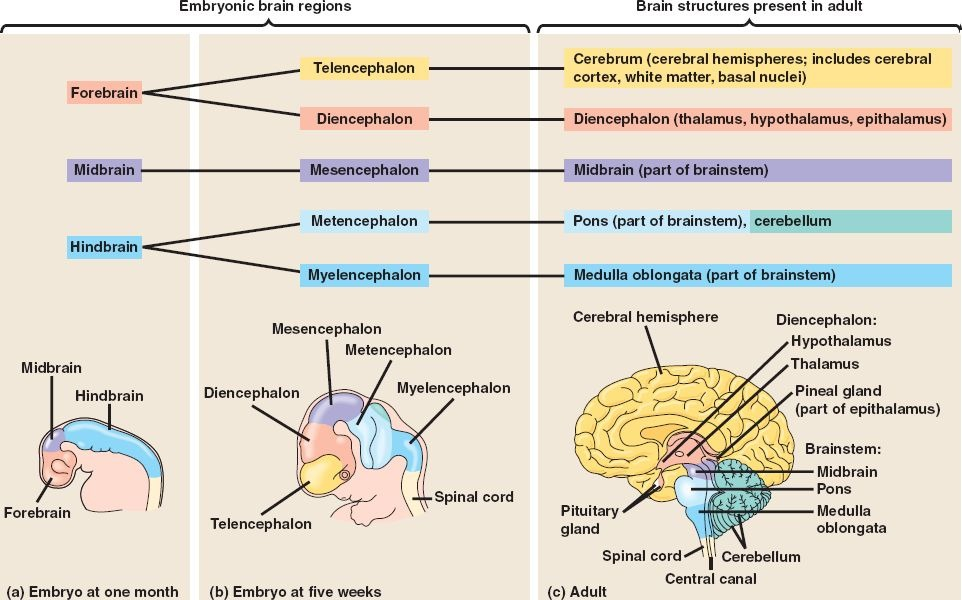
\includegraphics[width=0.5\textwidth]{assets/development.png}
    \caption{Brain development}
    \end{figure}
    
    \noindent Forebrain (Prosencephalon) which can be further sub-divided into:
    \begin{itemize}
        \item Telencephalon: develops into the cerebral cortex, basal ganglia, hippocampal formation, amygdala
        \item Diencephalon: gives rise to structures like the thalamus, hypothalamus and the pituitary gland.
    \end{itemize}
    
    \noindent Midbrain (Mesencephalon) tectum and tegmentum, which exist in all vertebrate brains. The tectum in the mammalian brain consists of the superior colliculus and the inferior colliculus.
    
    \noindent Hindbrain (Rhombencephalon) consists of the Metencephalon (develops into the pons, cerebellum) and the Myelencephalon (develops into the medulla oblongata)
    
    \begin{figure}[H]
    \centering
    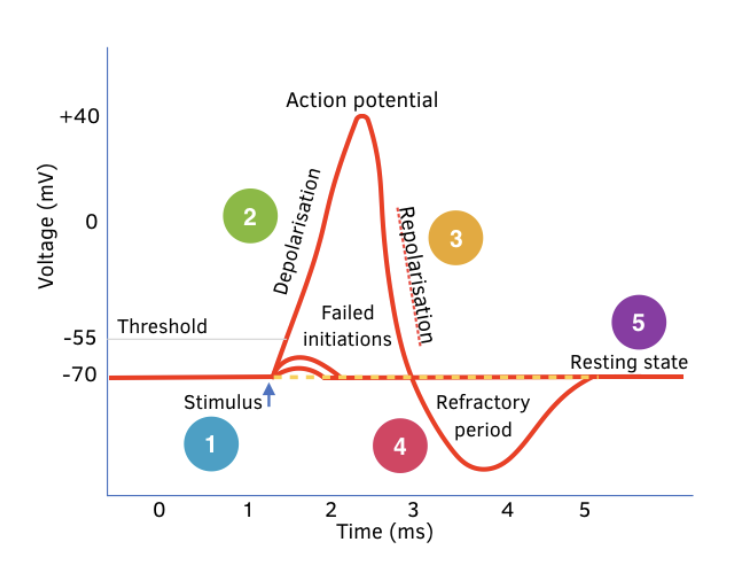
\includegraphics[width=0.5\textwidth]{assets/polarization.png}
    \caption{Neuron polarization}
    \end{figure}
    
    \noindent Neurons are hyperpolarized which means they have a resting potential of -70 mV within and 0 mV outside of them. Hyperpolarization refers to an increase in membrane potential whereas depolarization refers to a decrease in membrane potential
    
    \noindent Action potentials are all or nothing operations which have four components which take place over the course of 1-2 ms:
    Depolarization: Depolarization is when a change occurs inside a cell that causes the distribution of electric charges to alter, leaving the cell with a less negative charge than the outside. Numerous cell functions, cell-cell communication, and the general physiology of an organism all depend on depolarization
    

\section{Resting Potentials}

\subsection{Understanding Resting Membrane Potential}
\begin{itemize}
    \item The resting membrane potential is a fundamental property of neurons, typically around -70 mV in mammals. 
    \item It is crucial for neuron excitability and forms the basis for action potentials.
\end{itemize}

\subsection{Ion Distribution and Membrane Permeability}
\begin{itemize}
    \item The resting potential is established by the uneven distribution of ions across the cell membrane and the selective permeability of the membrane to certain ions.
    \item Key ions include potassium (K+), sodium (Na+), chloride (Cl-), and calcium (Ca2+).
\end{itemize}
Ion distribution and membrane permeability are essential concepts in cellular biology and neuroscience. These concepts play a fundamental role in understanding various physiological processes, including the resting membrane potential, action potentials in neurons, and the functioning of ion channels.

\subsubsection{Ion Distribution}

Intracellular and extracellular fluids contain different concentrations of ions, which contribute to various cellular processes. Key ions involved include:

\subsubsection{Sodium (Na$^+$)}

\begin{itemize}
  \item Sodium ions are more concentrated in the extracellular fluid.
  \item They play a crucial role in depolarizing the cell membrane during an action potential.
\end{itemize}

\subsubsection{Potassium (K$^+$)}

\begin{itemize}
  \item Potassium ions are more concentrated in the intracellular fluid.
  \item They are primarily responsible for maintaining the resting membrane potential.
\end{itemize}

\subsubsection{Calcium (Ca$^{2+}$)}

\begin{itemize}
  \item Calcium ions are also more concentrated in the extracellular fluid.
  \item They are involved in various cellular processes, including neurotransmitter release and muscle contraction.
\end{itemize}

\subsubsection{Membrane Permeability}

The cell membrane is selectively permeable, allowing certain ions to pass through while restricting the movement of others. Membrane permeability is regulated by various factors, including:

\paragraph{Ion Channels}

\begin{itemize}
  \item Ion channels are integral membrane proteins that facilitate the selective passage of specific ions.
  \item They can be voltage-gated, ligand-gated, or mechanically gated, depending on their mode of regulation.
\end{itemize}

\subsubsection{Ion Pumps}

\begin{itemize}
  \item Ion pumps, such as the sodium-potassium pump (Na$^+$/K$^+$ pump), actively transport ions against their concentration gradients.
  \item These pumps are essential for maintaining the ion distribution required for neuronal excitability and other cellular functions.
\end{itemize}

\subsubsection{Resting Membrane Potential}

The resting membrane potential is the electrical charge difference across a cell membrane when the cell is at rest. It is primarily determined by the permeability of the membrane to potassium ions, which are more concentrated inside the cell. This results in a negative charge inside the cell compared to the extracellular fluid. The resting membrane potential is typically around -70 millivolts in neurons.

\subsubsection{Action Potentials}

Action potentials are rapid changes in membrane potential that allow neurons to transmit electrical signals. They occur when there is a sudden increase in membrane permeability to sodium ions, followed by a subsequent increase in potassium ion permeability. This sequence of events leads to depolarization and repolarization of the cell membrane.

\subsubsection{Conclusion}

Ion distribution and membrane permeability are fundamental concepts in cellular biology and neuroscience. Understanding how ions move across cell membranes and how membrane permeability is regulated is crucial for comprehending processes like the resting membrane potential and action potentials in neurons, which are essential for information transmission in the nervous system.



\subsection{Nernst Equation}
\begin{itemize}
    \item The Nernst equation calculates the equilibrium potential for a single ion based on its concentration gradient across the membrane.
    \item It helps in understanding how the concentration gradients of individual ions contribute to the resting membrane potential.
\end{itemize}
The Nernst equation is a fundamental equation in electrochemistry and physiology that describes the relationship between the electrical potential (voltage) across a cell membrane and the concentration gradient of a specific ion. It is commonly used to calculate the equilibrium potential for a particular ion across a semi-permeable membrane, such as a cell membrane.

The Nernst equation is represented as follows:

\[
E = \frac{RT}{zF} \ln\left(\frac{[X]_{\text{outside}}}{[X]_{\text{inside}}}\right)
\]

Where:
\begin{itemize}
  \item \(E\) represents the equilibrium potential (in volts, V) for the ion of interest.
  \item \(R\) is the universal gas constant (\(8.314 \, \text{J/mol} \cdot \text{K}\)).
  \item \(T\) is the absolute temperature in Kelvin (K).
  \item \(z\) is the charge of the ion (e.g., +1 for potassium ions, -1 for chloride ions).
  \item \(F\) is Faraday's constant (\(96,485 \, \text{C/mol}\)).
  \item \([X]_{\text{outside}}\) is the concentration of the ion outside the cell membrane (in mol/L).
  \item \([X]_{\text{inside}}\) is the concentration of the ion inside the cell membrane (in mol/L).
\end{itemize}

The Nernst equation provides a way to calculate the equilibrium potential for a specific ion when the ion's concentrations on either side of the membrane are known. When the electrical potential (\(E\)) equals the equilibrium potential for an ion, there is no net movement of that ion across the membrane, and the system is said to be in electrochemical equilibrium.

The Nernst equation is particularly important in neuroscience and cellular physiology, as it helps explain how the resting membrane potential of neurons is established and how changes in ion concentrations can affect neuronal excitability. For example, the Nernst equation can be used to calculate the resting membrane potential of a neuron based on the concentrations of sodium (\(Na^+\)), potassium (\(K^+\)), and chloride (\(Cl^-\)) ions both inside and outside the cell.


\subsection{Goldman-Hodgkin-Katz Equation}
\begin{itemize}
    \item This equation extends the Nernst equation to consider multiple ions. 
    \item It provides a more accurate representation of the resting membrane potential, accounting for the relative permeabilities of different ions.
\end{itemize}
The Goldman-Hodgkin-Katz equation, often referred to as the GHK equation, is a critical tool in the field of physiology and biophysics. It builds upon the principles of the Nernst equation and allows for the calculation of the resting membrane potential (\(V_{\text{rest}}\)) and the ionic currents across cell membranes, especially in excitable cells like neurons.

\subsubsection{The GHK Equation}

The GHK equation is formulated as follows:

\[
V_{\text{rest}} = \frac{RT}{F} \ln \left(\frac{\sum_i P_i[\text{ion}_i]_{\text{out}}}{\sum_i P_i[\text{ion}_i]_{\text{in}}}\right)
\]

Where:
\begin{itemize}
  \item \(V_{\text{rest}}\) is the resting membrane potential (in volts, V).
  \item \(R\) is the universal gas constant (\(8.314 \, \text{J/mol} \cdot \text{K}\)).
  \item \(T\) is the absolute temperature in Kelvin (K).
  \item \(F\) is Faraday's constant (\(96,485 \, \text{C/mol}\)).
  \item \(\sum_i\) represents the summation over all relevant ions.
  \item \(P_i\) is the permeability of the membrane to the ion \(i\).
  \item \([\text{ion}_i]_{\text{out}}\) is the concentration of ion \(i\) outside the cell membrane (in mol/L).
  \item \([\text{ion}_i]_{\text{in}}\) is the concentration of ion \(i\) inside the cell membrane (in mol/L).
\end{itemize}

The GHK equation is more comprehensive than the Nernst equation as it considers the permeabilities (\(P_i\)) of multiple ions and their respective concentration gradients. This allows for a more accurate calculation of the resting membrane potential, taking into account the relative contribution of each ion.

\subsubsection{Significance}

The Goldman-Hodgkin-Katz equation is particularly important in the study of excitable cells like neurons, where the resting membrane potential and the propagation of action potentials are vital for information processing. By considering the permeabilities of sodium (\(Na^+\)), potassium (\(K^+\)), and other ions, the GHK equation provides a more realistic representation of the membrane potential compared to the simpler Nernst equation. It helps elucidate the complex interplay of ions in cellular physiology.

\subsubsection{Conclusion}

The Goldman-Hodgkin-Katz equation is a powerful tool for understanding the resting membrane potential and ionic currents in excitable cells. Its extension of the Nernst equation by incorporating permeabilities of multiple ions makes it invaluable in the field of physiology and biophysics, especially in elucidating the mechanisms of neuronal excitability.
\begin{figure}[H]
\centering
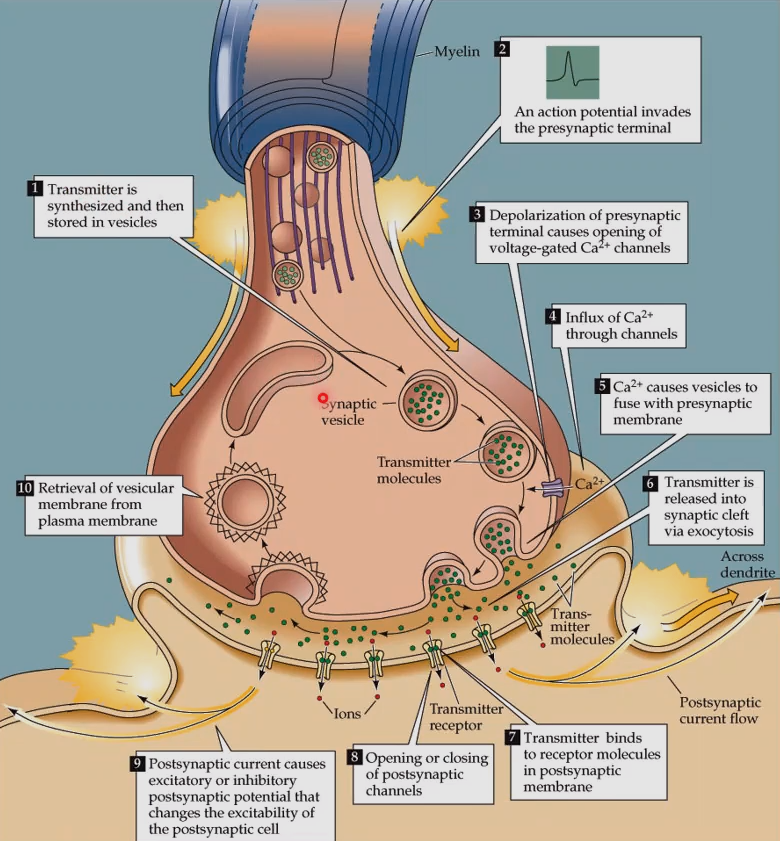
\includegraphics[width=0.5\textwidth]{assets/chemical-synapses.png}
\caption{Chemical synapses}
\end{figure}

\subsection{Chemical transmission}

\begin{itemize}
    \item Contrary to electrical transmission multiple steps are required to release transmitter chemicals and for them to act on postsynaptic receptors, resulting in a time delay
    \item Directional, select localization of release machinery to presynaptic terminals and receptors to postsynaptic specializations
    \item can change sign by release of inhibitory transmitter
    \item highly modulatable as it has many steps presynaptic terminal and at the postsynaptic sites
\end{itemize}

\begin{figure}[H]
\centering
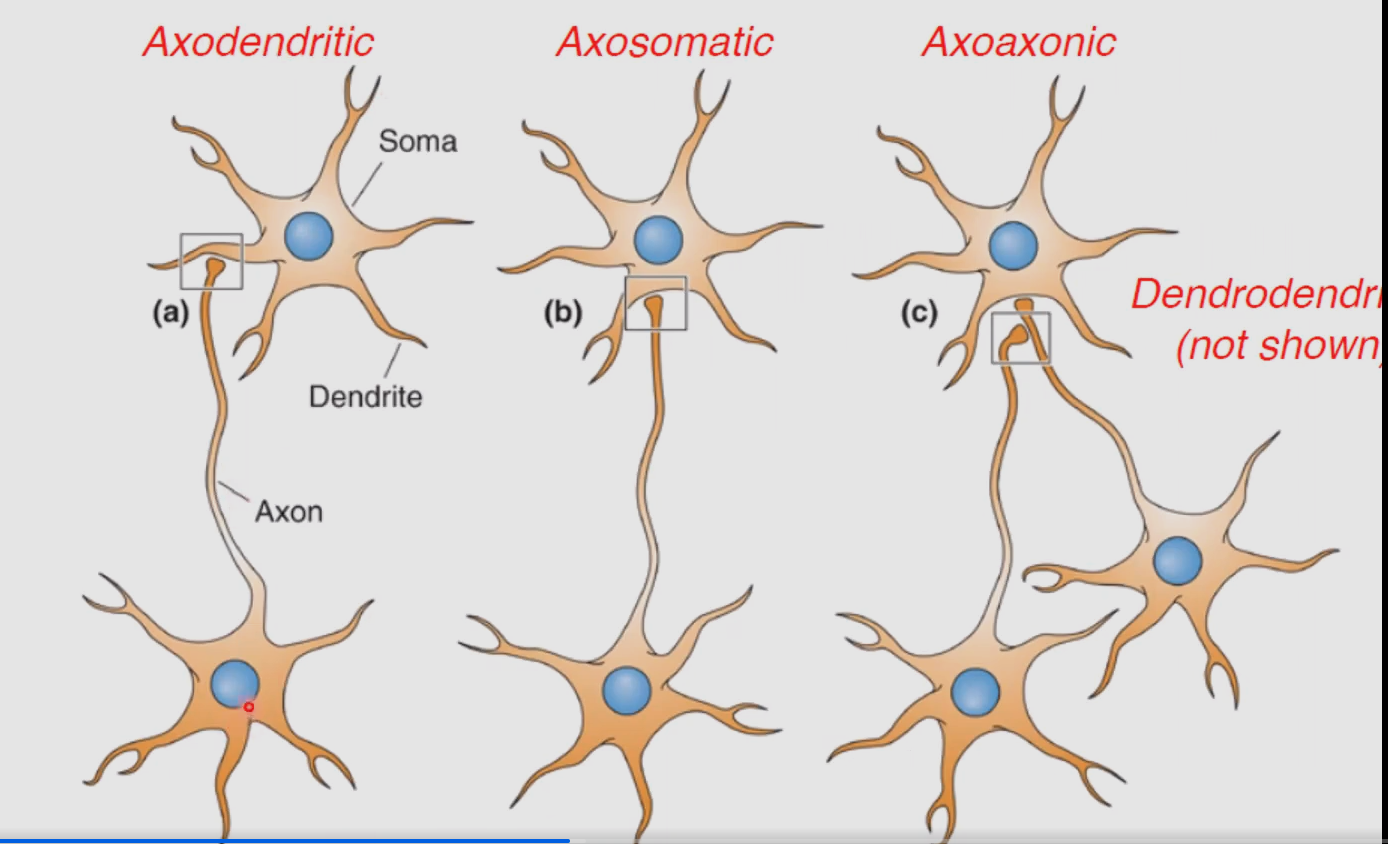
\includegraphics[width=0.5\textwidth]{assets/types-of-synapses.png}
\caption{Types of synapses}
\end{figure}

\subsection{Steps to chemical synaptic transmission}

\begin{itemize}
    \item First need to bring the presynaptic neuron to threshold at axon hillock
    \item Conduction down axon length $R * C$ dependent
    \item Opening of voltage gated Ca channels
    \item Diffusion and action of Ca at release machinery
    \item Exocytosis and diffusion of transmitter in cleft
    \item Activation of postsynaptic receptors
\end{itemize}

\subsection{Criteria that define a neurotransmitter}

\begin{enumerate}
    \item must be present at presynaptic terminal
    \item must be released by depolarization, $Ca^{++}$-dependent
    \item specific receptors must be present
\end{enumerate}

\begin{figure}[H]
\centering
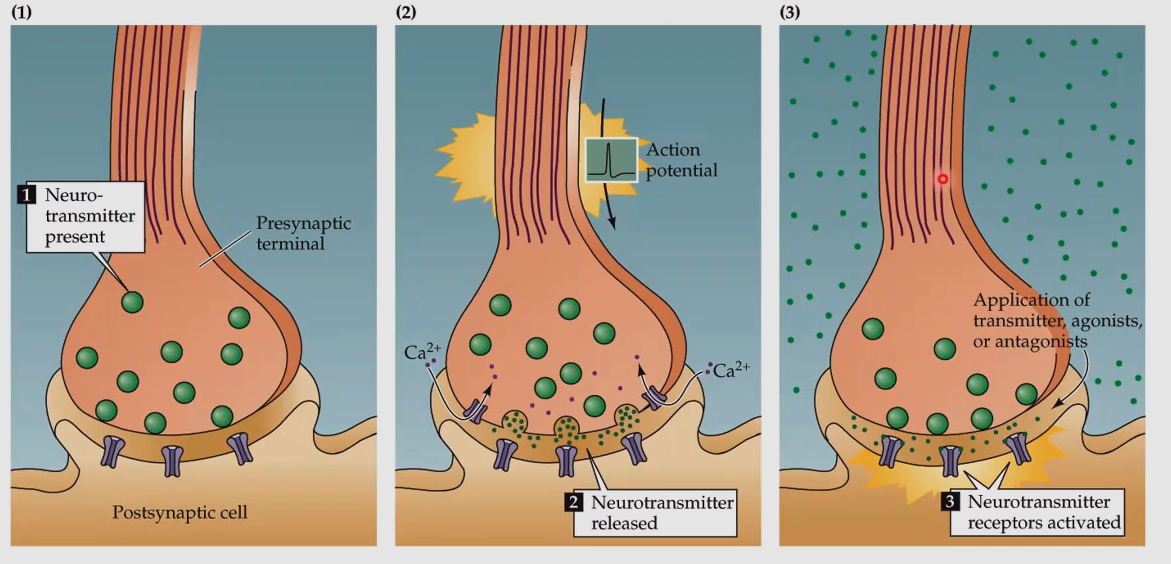
\includegraphics[width=0.5\textwidth]{assets/neurotransmitter.png}
\caption{Neurotransmitter}
\end{figure}

\subsection{Standard Katz (Quantal) Model of Synaptic Transmission}

\begin{itemize}
    \item One packet of neurotransmitter = 1 quantum
    \item AP transiently increases in the probability of releasing NX quanta
    \item Several quanta are available to be released
    \item Each quantum gives approximately the same postsynaptic response called the Quantal Amplitude
    \item The average number of quanta released, $m = np$
      \begin{itemize}
        \item where $n$ = number of quanta available for release
        \item $p$ = their average release probability
      \end{itemize}
\end{itemize}

\subsection{CNS synapses and quanta}

\begin{itemize}
    \item at CNS synapses with only a single release site, changing the probability of release (i.e. changing calcium concentration) does not effect the amplitude of the response (as only zero or one vesicle is released in theory)
    \item at CNS synapses with multiple release sites, changing release probability can change the postsynaptic response amplitude as more transmitter is released (graded quantal levels)
    \item at the NMJ a single nerve can elicit a postsynaptic AP given multiquantal release, while at the CNS synapse (with low number of release sites) multiple synapses must cooperate, forces a network
\end{itemize}

\subsection{Docked Synaptic Vesicles}

Define the number of readily releasable vesicles a synapse has available. A consequence of having of limited number is depletion at high stimulus frequency, CNS synapses may have only a small number of docked vesicles on the order of 5-10 vesicles for a hippocampal CA1 synapse

\begin{figure}[H]
\centering
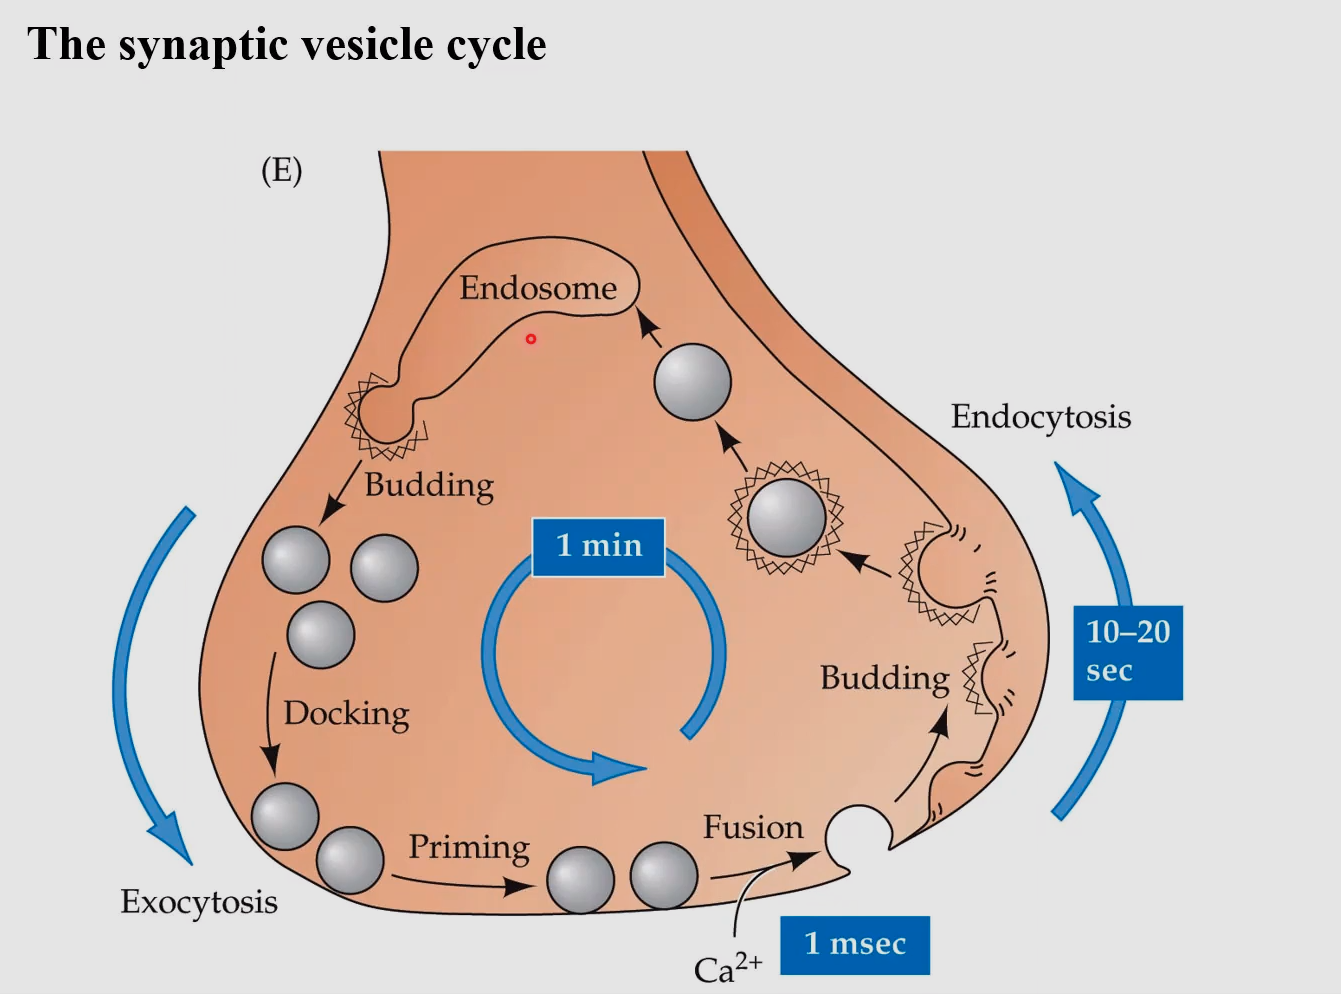
\includegraphics[width=0.5\textwidth]{assets/synaptic-vesicle-cycle.png}
\caption{Synaptic vesicle cycle}
\end{figure}

\subsection{Ion Channels and Pumps}
\begin{itemize}
    \item Ion channels allow specific ions to pass through the membrane, contributing to the resting potential.
    \item Ion pumps, such as the sodium-potassium pump, actively maintain ion concentration gradients, crucial for the long-term stability of the resting potential.
\end{itemize}

\subsection{Biophysical Implications}
\begin{itemize}
    \item Understanding the resting potential is key to comprehending how neurons encode and transmit information.
    \item It sets the stage for exploring how changes in membrane potential lead to various forms of neural signaling.
\end{itemize}
\section{Passive Membrane Properties}

\subsection{Electrical Properties of Neuronal Membranes}
\begin{itemize}
    \item The neuronal membrane can be modeled as an electrical circuit with resistors and capacitors representing its ion channels and lipid bilayer, respectively.
    \item Membrane resistance (Rm) affects the flow of ionic currents, with high resistance leading to less leakage of ions and a more extended influence of synaptic inputs.
    \item Membrane capacitance (Cm) reflects the membrane's ability to store and release charge, influencing how quickly the membrane potential can change in response to synaptic inputs.
\end{itemize}

\subsection{Role of Dendrites in Signal Transmission}
\begin{itemize}
    \item Dendrites, with their branched structures, receive input from other neurons. Their geometry and passive properties significantly influence how these inputs are integrated and transmitted to the neuron's cell body.
    \item Passive signal spread in dendrites is a function of the membrane and cytoplasmic resistance and the membrane capacitance.
\end{itemize}

\subsection{Importance of Axonal Properties}
\begin{itemize}
    \item Axons, especially myelinated ones, are critical for the rapid conduction of signals over long distances.
    \item Myelin, a fatty substance that wraps around axons, increases conduction speed by reducing membrane capacitance and increasing membrane resistance.
\end{itemize}

\subsection{Synaptic Currents and Integration}
\begin{itemize}
    \item Synaptic currents are generated by neurotransmitter release and subsequent receptor activation. These currents can be excitatory or inhibitory, influencing the postsynaptic neuron's membrane potential.
    \item The integration of these currents is a complex process influenced by the dendritic structure and the distribution of ion channels.
\end{itemize}

\subsection{Cable Theory and Its Implications}
\begin{itemize}
    \item Cable theory models the passive flow of currents along dendrites and axons, providing insights into how electrical signals decay over distance and time.
    \item It helps in understanding the length constant and time constant, which are measures of how far and how quickly signals can passively spread in neural processes.
\end{itemize}


Cable theory is a foundational concept in the fields of neuroscience and biophysics, which provides a framework for understanding how electrical signals propagate through biological structures like neurons, dendrites, and axons. It allows us to model and analyze the electrical properties of these complex structures and has important implications for our understanding of neural signal transmission.

\subsubsection{Cable Equation}

The cable equation is a partial differential equation that describes the distribution of electrical potential (\(V\)) along a cylindrical cable-like structure. It is typically used to model the behavior of dendrites and axons in neurons. The cable equation can be represented as:

\[
\lambda^2 \frac{{\partial^2 V}}{{\partial x^2}} = \frac{{\partial V}}{{\partial t}} - R_m \cdot I_m
\]

Where:
\begin{itemize}
  \item \(\lambda\) represents the length constant, which is a measure of how far an electrical signal can propagate along the cable before it attenuates significantly.
  \item \(\frac{{\partial V}}{{\partial x}}\) is the spatial gradient of the electrical potential along the cable.
  \item \(\frac{{\partial V}}{{\partial t}}\) is the temporal change in electrical potential.
  \item \(R_m\) is the membrane resistance, which quantifies how easily ions can flow across the neuronal membrane.
  \item \(I_m\) is the transmembrane current, representing the net flow of ions across the membrane.
\end{itemize}

\subsubsection{Implications}

Cable theory has several important implications for our understanding of neural physiology and signal transmission:

\subsubsection{Signal Attenuation}

Cable theory helps us understand how electrical signals attenuate as they propagate along dendrites and axons. The length constant (\(\lambda\)) determines the spatial extent over which a signal remains relatively strong. Longer dendrites or axons may require specialized mechanisms to boost or regenerate signals.

\subsubsection{Synaptic Integration}

Neurons receive inputs from multiple sources via synapses on their dendrites. Cable theory helps us analyze how these synaptic inputs integrate spatially and temporally. The electrical properties of dendrites influence how synaptic inputs are summed and affect the neuron's firing pattern.

\subsubsection{Action Potential Propagation}

Cable theory aids in our understanding of action potential propagation along axons. The cable equation can be used to calculate the critical length and diameter required for the successful propagation of action potentials. It also highlights the importance of myelination in reducing capacitive and resistive losses.

\subsubsection{Neuronal Excitability}

The membrane resistance (\(R_m\)) and membrane capacitance (\(C_m\)) values derived from cable theory help quantify the electrical excitability of neurons. Neurons with high \(R_m\) values require larger synaptic inputs to reach the threshold for action potential initiation.

\subsubsection{Conclusion}

Cable theory is a foundational concept in neuroscience and biophysics that provides a framework for understanding electrical signal propagation in complex biological structures. Its implications extend to synaptic integration, action potential propagation, and the electrical properties of neurons, contributing significantly to our understanding of neural function and communication.


\subsection{Applications in Understanding Neuronal Function}
\begin{itemize}
    \item The study of passive membrane properties is essential in interpreting how neurons respond to synaptic inputs and contribute to neural network dynamics.
    \item This understanding is crucial for developing models of neural circuits and for designing neural prosthetics and brain-computer interfaces.
\end{itemize}

\section{Action Potential}

\subsection{Basics of Action Potential}
\begin{itemize}
    \item An action potential is a rapid, transient change in the membrane potential of a neuron.
    \item It is an all-or-none event, meaning it occurs fully or not at all, and is critical for neural communication.
\end{itemize}

\subsection{Phases of Action Potential}
\begin{enumerate}
    \item Resting state: The neuron is at its resting potential, typically around -70mV.
    \item Depolarization: Upon receiving a sufficient stimulus, sodium channels open, causing a rapid influx of Na+ ions and a rise in membrane potential.
    \item Repolarization: As the potential reaches its peak, sodium channels close, and potassium channels open, allowing K+ ions to flow out, bringing the membrane potential back down.
    \item Hyperpolarization: The membrane potential temporarily becomes more negative than the resting potential, due to the continued efflux of K+ ions.
    \item Return to resting state: Ion concentrations are restored to their original state by the sodium-potassium pump.
\end{enumerate}

\subsection{Ionic Basis of Action Potential}
\begin{itemize}
    \item The action potential is driven by the movement of ions across the neuronal membrane through voltage-gated ion channels.
    \item The differential permeability of the membrane to Na+ and K+ ions, controlled by these channels, is critical for the generation and propagation of action potentials.
\end{itemize}

\subsection{Hodgkin and Huxley's Contributions}
\begin{itemize}
    \item Hodgkin and Huxley developed the voltage clamp technique and used it to study the ionic currents during action potentials in the squid giant axon.
    \item Their work led to a detailed understanding of how voltage-gated Na+ and K+ channels contribute to the action potential, earning them a Nobel Prize.
\end{itemize}

\subsection{Refractory Periods}
\begin{itemize}
    \item Following an action potential, the neuron enters a refractory period, during which it is less likely or unable to generate another action potential.
    \item The refractory period ensures unidirectional propagation of the action potential and limits the frequency of action potentials.
\end{itemize}

\subsection{Implications for Neural Communication}
\begin{itemize}
    \item Action potentials are fundamental for neural communication, allowing neurons to transmit signals over long distances.
    \item The frequency and pattern of action potentials encode information in the nervous system.
\end{itemize}

\section{Synapses 1}

\subsection{Discovery and Historical Perspective}
\begin{itemize}
    \item Synaptic transmission was first hypothesized in the early 1900s, with significant contributions by scientists like Cajal and Sherrington.
    \item Otto Loewi's experiments in the 1930s provided strong evidence for chemical neurotransmission.
\end{itemize}

\subsection{Chemical Synaptic Transmission}
\begin{itemize}
    \item Chemical transmission involves neurotransmitters released from the presynaptic neuron and binding to receptors on the postsynaptic neuron.
    \item This process is essential for communication between neurons and is characterized by synaptic delays.
\end{itemize}

\subsection{Criteria for Neurotransmitters}
\begin{itemize}
    \item Neurotransmitters must be present in the presynaptic terminal, released upon depolarization, and specific receptors must be present on the postsynaptic neuron.
    \item They can be small molecules or peptides with different synthesis and release mechanisms.
\end{itemize}

\subsection{Role of Calcium in Neurotransmitter Release}
\begin{itemize}
    \item Calcium influx through voltage-gated channels triggers the release of neurotransmitters.
    \item The amount and timing of calcium entry are crucial for the regulation of neurotransmitter release.
\end{itemize}

\subsection{The Synaptic Vesicle Cycle}
\begin{itemize}
    \item The cycle includes docking, priming, and fusion of synaptic vesicles with the presynaptic membrane.
    \item Proteins like SNAREs and NSF are involved in this process, facilitating the release of neurotransmitters.
\end{itemize}

\subsection{Quantal Release and Miniature Events}
\begin{itemize}
    \item Neurotransmitter release occurs in discrete packets or quanta.
    \item Miniature postsynaptic potentials represent the release of single vesicles and are important for understanding synaptic function and plasticity.
\end{itemize}

\section{Synapses 2}

\subsection{The Synaptic Vesicle Cycle}
\begin{itemize}
    \item The cycle involves multiple steps: docking, priming, fusion, and retrieval of synaptic vesicles.
    \item Docking: Vesicles prepare for release by attaching to the presynaptic membrane.
    \item Priming: Vesicles are readied for neurotransmitter release, a process regulated by various proteins and calcium levels.
    \item Fusion: Vesicles release their neurotransmitter content into the synaptic cleft.
    \item Retrieval: Following fusion, vesicles are reformed and recycled.
\end{itemize}

\subsection{Molecular Mechanisms of Vesicle Release}
\begin{itemize}
    \item Proteins such as SNAREs and NSF are integral in the docking and fusion of synaptic vesicles.
    \item The SNARE complex facilitates the merging of vesicle and membrane lipids, leading to neurotransmitter release.
\end{itemize}

\subsection{Electrical and Chemical Synapses}
\begin{itemize}
    \item Electrical synapses involve gap junctions that allow direct electrical communication between neurons.
    \item Chemical synapses rely on neurotransmitter release and are the more common type of synaptic transmission.
    \item The differences in speed, flexibility, and functionality between these two types of synapses are critical for various neural processes and signaling.
\end{itemize}

\subsection{Quantal Release and Synaptic Efficacy}
\begin{itemize}
    \item Neurotransmitter release is quantal, meaning it occurs in discrete packets.
    \item The strength and efficacy of a synaptic connection depend on the number of vesicles released and the sensitivity of the postsynaptic receptors.
\end{itemize}

\subsection{Synaptic Plasticity}
\begin{itemize}
    \item Synaptic plasticity refers to the ability of synapses to strengthen or weaken over time, crucial for learning and memory.
    \item Mechanisms like long-term potentiation (LTP) and long-term depression (LTD) are examples of synaptic plasticity.
\end{itemize}
\section{The Neural Code}

\subsection{Introduction to Neural Coding}
\begin{itemize}
    \item Neural coding is the study of how the brain encodes and decodes information.
    \item Understanding neural coding is key to deciphering how thoughts, actions, and perceptions are represented in the brain.
\end{itemize}

\subsection{Rate Coding vs. Temporal Coding}
\begin{itemize}
    \item Rate coding refers to the hypothesis that information is encoded in the firing rate of neurons.
    \item Temporal coding suggests that timing patterns in spike trains carry information.
\end{itemize}

\subsection{Models of Neural Response to Stimuli}
\begin{itemize}
    \item Neural responses to stimuli can be modeled to understand how sensory information is processed.
    \item Examples include Hubel and Wiesel's studies on orientation-selective neurons in the visual cortex.
\end{itemize}

\subsection{Encoding of Motor Output}
\begin{itemize}
    \item The motor cortex encodes information necessary for movement planning and execution.
    \item Georgopoulos' work demonstrated that the direction of arm movements is encoded in the activity patterns of motor cortex neurons.
\end{itemize}

\subsection{Population Coding}
\begin{itemize}
    \item Population coding involves understanding how groups of neurons work together to represent information.
    \item It is essential for interpreting complex neural signals, like those in spatial navigation by hippocampal place cells.
\end{itemize}

\subsection{Stimulus-Response Relationships}
\begin{itemize}
    \item Understanding the relationship between stimuli and neural responses is crucial for decoding the neural code.
    \item This involves studying how neurons in different brain areas respond to specific external inputs.
\end{itemize}

\subsection{Implications and Future Directions}
\begin{itemize}
    \item Advances in understanding the neural code have implications for developing brain-computer interfaces and treating neurological disorders.
    \item Future research will continue to unravel the complexities of how information is processed and represented in the brain.
\end{itemize}
\section{Learning and Plasticity}

\subsection{Introduction to Learning and Plasticity}
\begin{itemize}
    \item Plasticity is the brain's ability to change and adapt as a result of experience.
    \item Learning is the process through which new information is acquired and integrated.
\end{itemize}

\subsection{Why Plasticity and Learning are Essential}
\begin{itemize}
    \item They are fundamental for adapting to new environments, forming memories, and learning new skills.
    \item Plasticity is the biological basis of learning and memory.
\end{itemize}

\subsection{Defining Plasticity and Learning}
\begin{itemize}
    \item Plasticity refers to changes in neural connections and strengths in response to experiences.
    \item Learning involves acquiring and processing new information or skills through experience or practice.
\end{itemize}

\subsection{Temporal Scales of Plasticity}
\begin{itemize}
    \item Plasticity occurs on various temporal scales, from short-term changes like synaptic efficacy to long-term structural changes in neural networks.
\end{itemize}

\subsection{Substrates of Neural Plasticity}
\begin{enumerate}
    \item Network and Systems Plasticity: Changes at the network or system level, affecting how different brain regions interact.
    \item Cellular Plasticity and the Perceptron: Cellular changes, such as the strengthening or weakening of synaptic connections.
    \item Synaptic Plasticity and the Hebbian Synapse: Refers to the principle that 'neurons that fire together wire together', emphasizing the role of simultaneous activation in strengthening synaptic connections.
\end{enumerate}

\subsection{Applications and Implications}
\begin{itemize}
    \item Understanding learning and plasticity is crucial for developing treatments for brain injuries and neurodegenerative diseases.
    \item Insights into plasticity and learning have profound implications for artificial intelligence and machine learning.
\end{itemize}
\section{Neuromorphic VLSI}

\subsection{Goal of Neuromorphic Engineering}
\begin{itemize}
    \item The primary objective is to design intelligent, adaptive machines that interact with the environment, resembling brain functions.
\end{itemize}

\subsection{Technological Requirements}
\begin{itemize}
    \item Power efficiency, memory efficiency, real-time processing, low latency, and adaptability are crucial factors in neuromorphic engineering.
\end{itemize}

\subsection{Lessons from the Brain}
\begin{itemize}
    \item Neuromorphic systems are inspired by the brain's ability to exploit sparsity, ensure locality in processing and learning, and utilize event-based communication.
\end{itemize}

\subsection{Event-based Sensing and Processing}
\begin{itemize}
    \item Neuromorphic systems employ event-driven sensing, processing only relevant information as it occurs, similar to neural spike encoding in the brain.
\end{itemize}

\subsection{Neuromorphic Hardware}
\begin{itemize}
    \item Technologies like Resistive Random Access Memory (RRAM) are used for efficient, brain-like computing.
    \item Neuromorphic systems are designed to mimic brain's efficient information processing strategies, such as temporal computation and local event-based computation.
\end{itemize}

\subsection{Applications and Future Directions}
\begin{itemize}
    \item Neuromorphic VLSI has significant implications for robotics, wearable technology, and edge computing, offering solutions for energy-efficient, real-time data processing.
\end{itemize}


\section{Introduction to Synapses}
Synapses are the key junctions through which neurons communicate with each other. This section explores the fundamental aspects of synapses, their types, and their roles in neural communication.

\subsection{Definition and Importance}
A synapse is a structure that permits a neuron to pass an electrical or chemical signal to another neuron. Synapses are critical for the processing and transmission of neural information, forming the basis of neural circuits and brain function.

\subsection{Types of Synapses}
\begin{itemize}
    \item \textbf{Electrical Synapses:} Direct physical connections allowing electric currents to pass directly from one neuron to another.
    \item \textbf{Chemical Synapses:} Involve neurotransmitters crossing the synaptic cleft to transmit signals between neurons.
\end{itemize}

\section{Structure of Synapses}
This section details the anatomy of a typical synapse, differentiating between the pre-synaptic and post-synaptic neurons.

\subsection{Anatomy of a Synapse}
Detailed exploration of synaptic structures, including synaptic vesicles, neurotransmitter molecules, receptors, and the synaptic cleft.

\section{Synaptic Transmission}
Understanding the process of neurotransmitter release and action is crucial in neuroinformatics.

\subsection{Neurotransmitter Release}
Discussion of how action potentials trigger the release of neurotransmitters from synaptic vesicles into the synaptic cleft.

\subsection{Mechanisms of Neurotransmitter Action}
Elaboration on how neurotransmitters interact with receptors on the post-synaptic neuron, leading to various neural responses.

\section{Types of Neurotransmitters and their Roles}
This section covers major neurotransmitters and their specific functions in the nervous system.

\begin{itemize}
    \item \textbf{Acetylcholine:} Involved in muscle action, attention, and learning.
    \item \textbf{Dopamine:} Key in reward, motivation, and motor control.
    \item \textbf{Serotonin:} Affects mood, appetite, and sleep.
\end{itemize}

\section{Synaptic Plasticity}
Exploring the concepts of long-term potentiation (LTP) and long-term depression (LTD), and their roles in learning and memory.

\subsection{Long-Term Potentiation and Depression}
Detailed discussion on how repeated stimulation of synapses leads to LTP, enhancing synaptic strength, and LTD, which weakens synapses.

\section{Synaptic Disorders}
Overview of common diseases and disorders related to synaptic malfunction, including current research and treatment approaches.

\subsection{Neurodegenerative Diseases}
Discussion on diseases like Alzheimer's and Parkinson's, focusing on their relation to synaptic dysfunction.

\section{Conclusion and Summary}
Summarization of key concepts covered, emphasizing their significance in neuroinformatics and broader neurological understanding.

\noindent\textbf{A hopfield network has symmetric weights and 0 self-weights}

\begin{figure}[H]
\centering
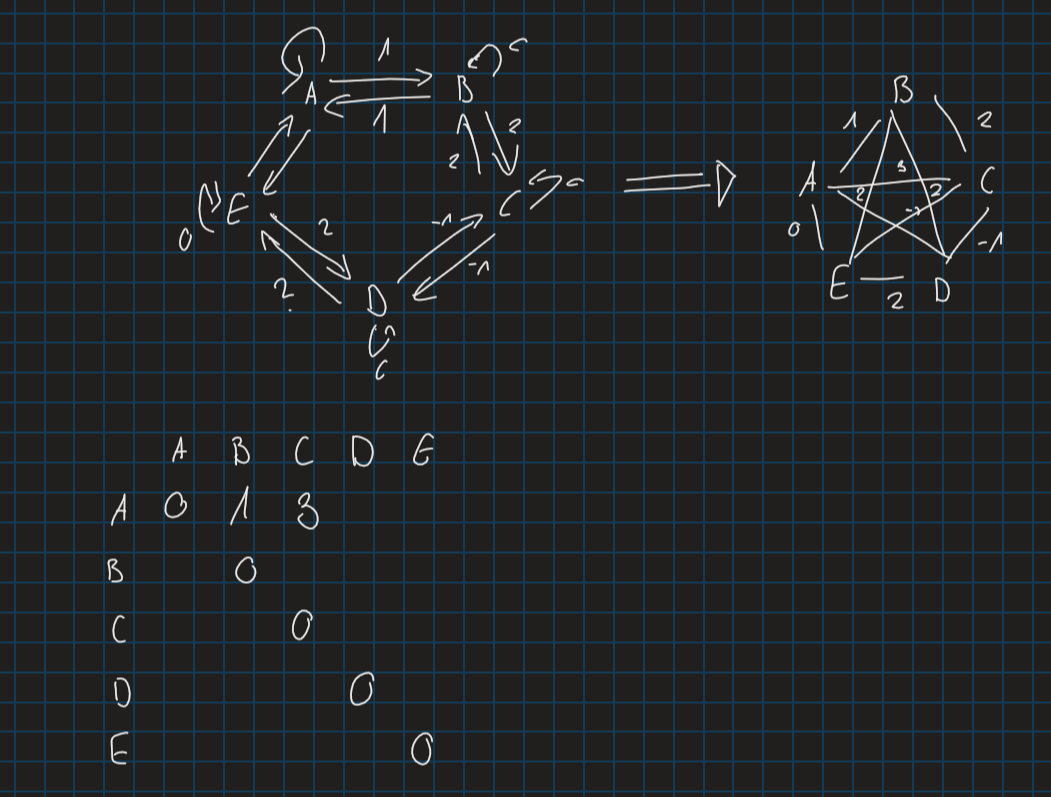
\includegraphics[width=0.5\textwidth]{assets/hopfieldNetwork.png}
\caption{Hopfield network}
\end{figure}

\noindent we update the state by updating a unit's output

\begin{center}
\begin{tabular}{ |c|c|c|c|c| }
\hline
A & B & C & D & E \\
\hline
1 & 1 & 0 & 0 & 0 \\
1 & 1 & 0 & 1 & 0 \\
1 & 1 & 0 & 1 & 1 \\
\hline
\end{tabular}
\end{center}

\noindent The state doesn't change after this (because every unit stays the same when updated) $\rightarrow$ the network has \textit{converged}

\begin{figure}[H]
\centering
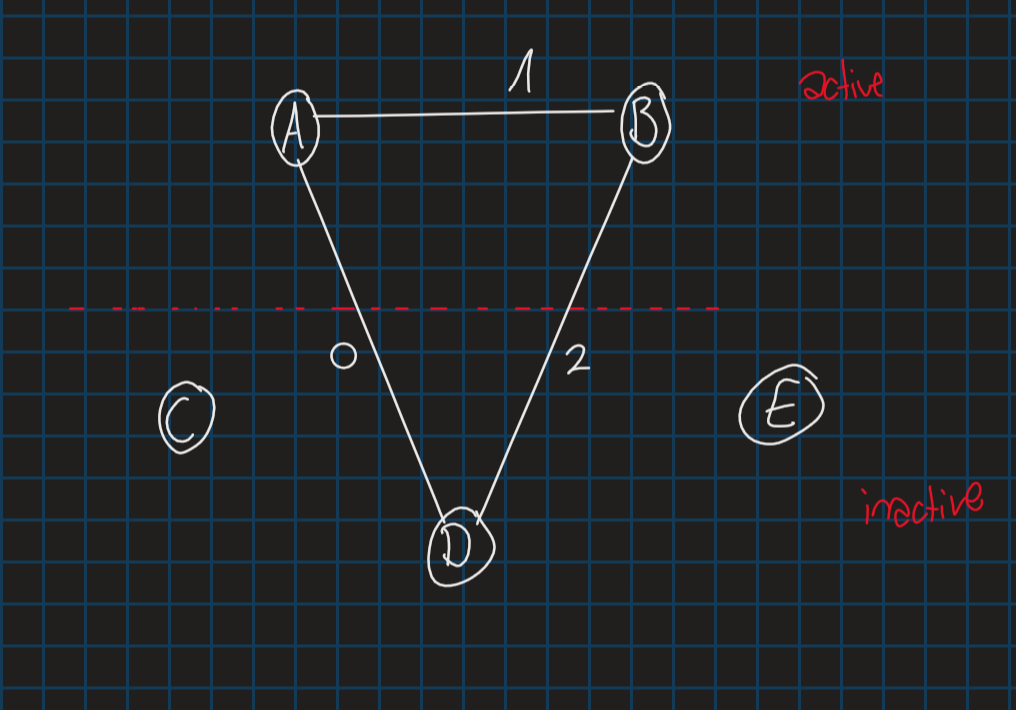
\includegraphics[width=0.5\textwidth]{assets/graph.png}
\caption{Graph}
\end{figure}

\noindent We move a unit to the top (bottom) if the sum of weights to \textit{upper} units is positive (negative)

\noindent Let's consider the sum of all weights between active units. This has to increase at every step. $\rightarrow$ every time we change the state of a unit.

\begin{figure}[H]
\centering
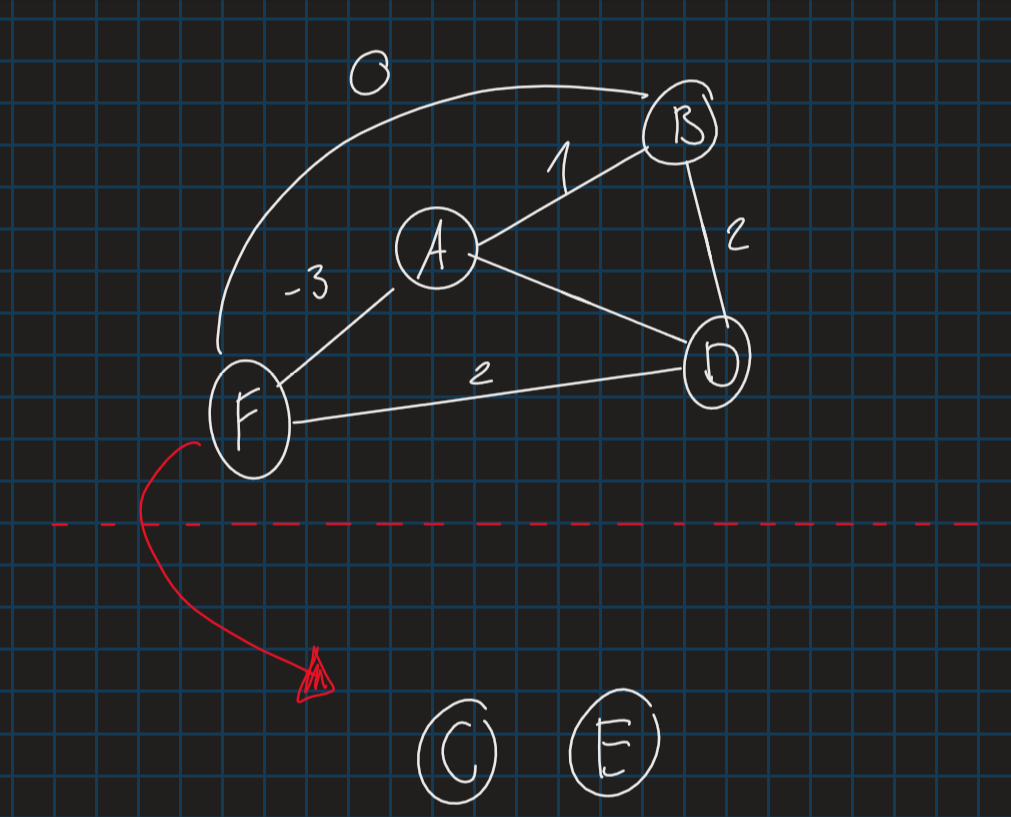
\includegraphics[width=0.5\textwidth]{assets/graph2.png}
\caption{Graph 2}
\end{figure}

\noindent Biased Graph:

\begin{figure}[H]
\centering
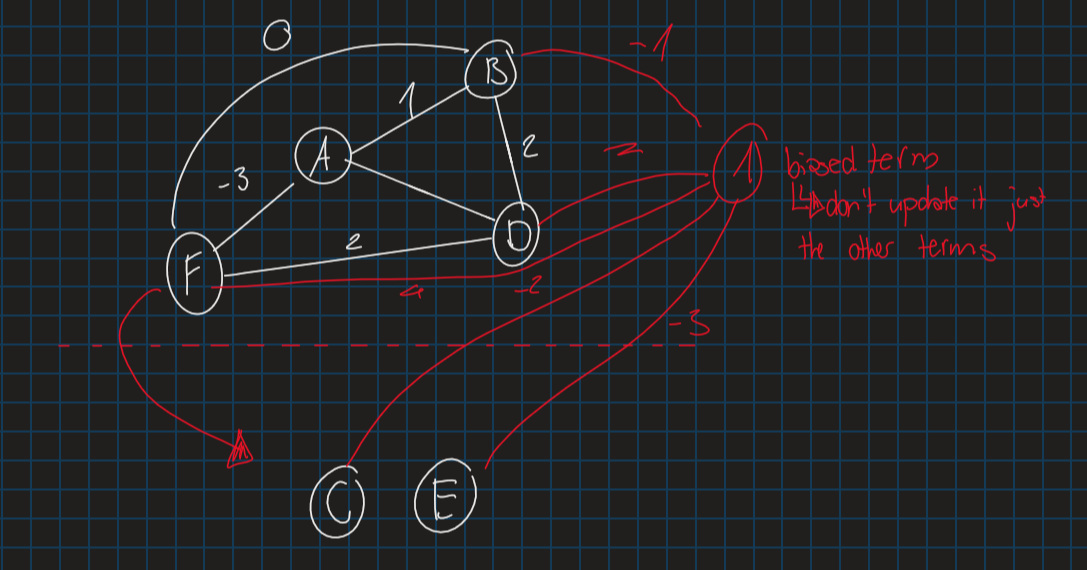
\includegraphics[width=0.5\textwidth]{assets/biasedGraph.png}
\caption{Biased graph}
\end{figure}

\noindent Even considering bias terms and cases where the threshold is reached exactly, the network has to converge to a stable state.

\section{Hopfield Network}

A hopfield network is an \textit{associative memory}\\
An associative memory restores a full memory from a partial or noisy version of the memory.

\subsection{Representations}

We can also use $\pm 1$ as the two states of a unit.

\begin{figure}[H]
\centering
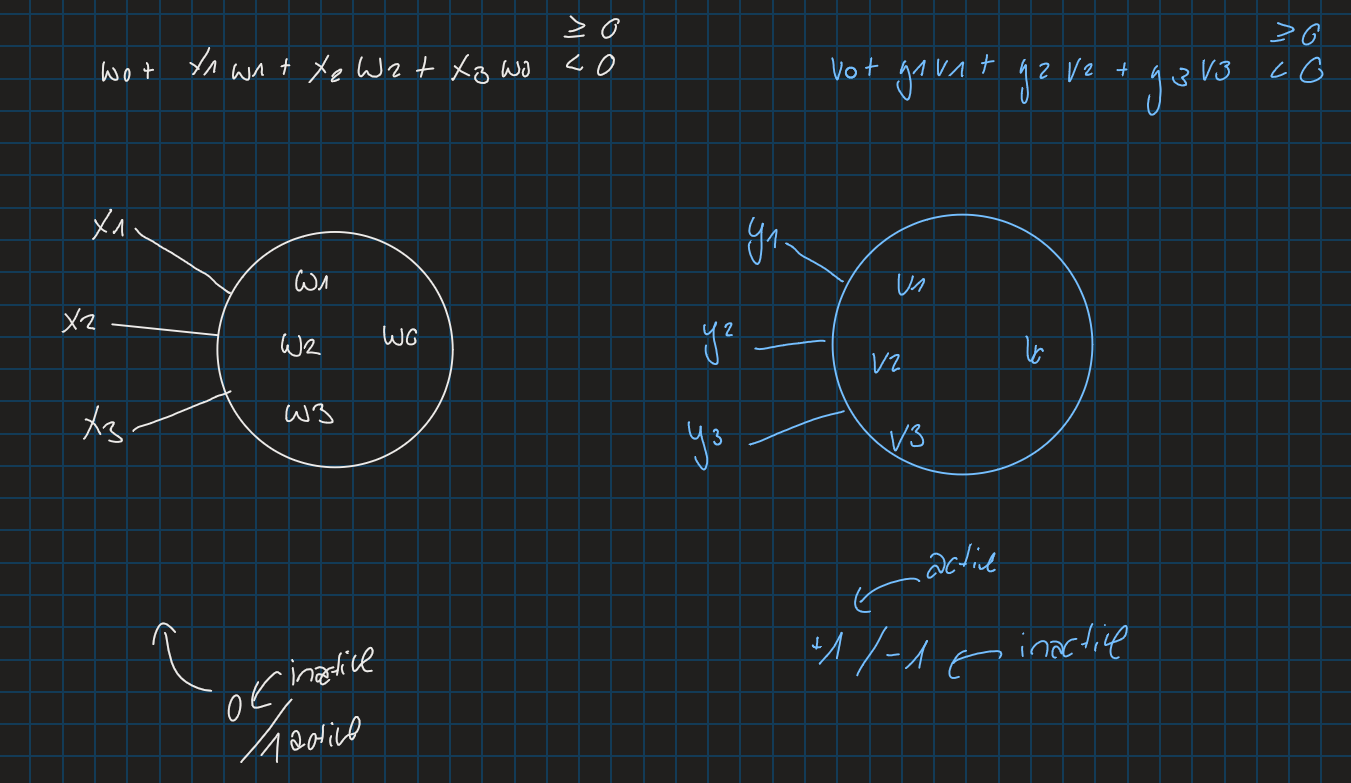
\includegraphics[width=0.5\textwidth]{assets/representation.png}
\caption{Representation}
\end{figure}

\begin{figure}[H]
\centering
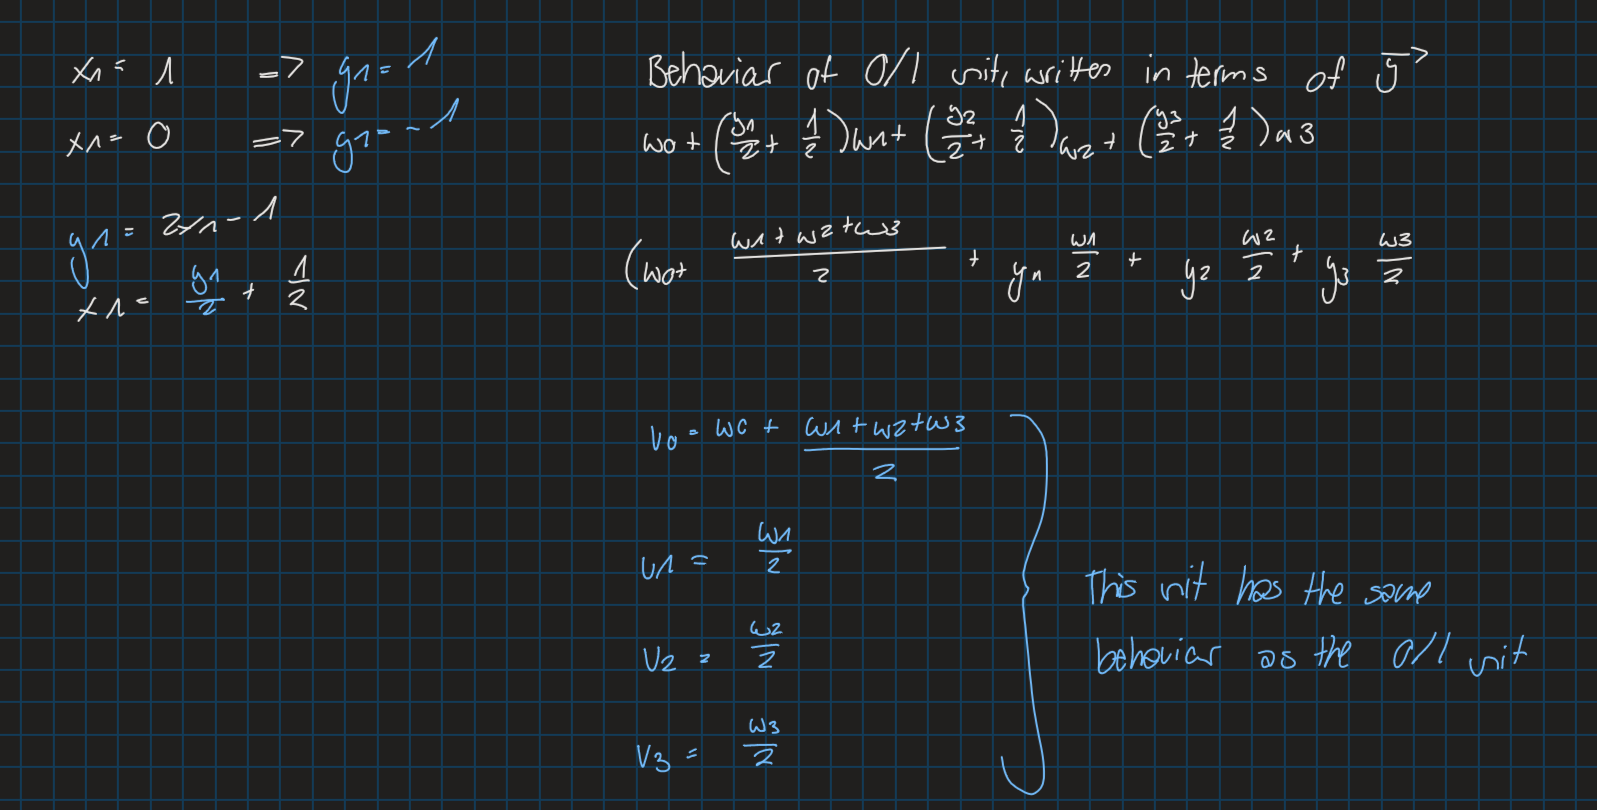
\includegraphics[width=0.5\textwidth]{assets/representation2.png}
\caption{Representation 2}
\end{figure}

\noindent So people don't worry about using one type vs the other - they use whichever they prefer.

\noindent \textbf{Asynchronous updates}: Updating units one at a time.

\noindent \textbf{Synchronous updates}: Updating all units simultaneously.

\noindent We can use our theorem about asynchronous networks to analyze synchronous ones. How?

\begin{center}
\begin{tabular}{ |c|c|c|c|c| }
\hline
A & B & C & D & E \\
\hline
1 & -1 & 1 & 1 & -1 \\
-1 & 1 & 1 & 1 & -1 \\
\hline
\end{tabular}
\end{center}


\subsection{Population Codes}

\begin{itemize}
    \item Neurons work together to encode a value or multiple values
    \item Each neuron is "tuned" to a particular value of the stimulus
    \item By looking at the activity of the population, the value is easy to read out.
\end{itemize}

\subsubsection{Example}



Neurons tuned to possible angles of a line at a certain location in the visual field.

\begin{figure}[H]
\centering
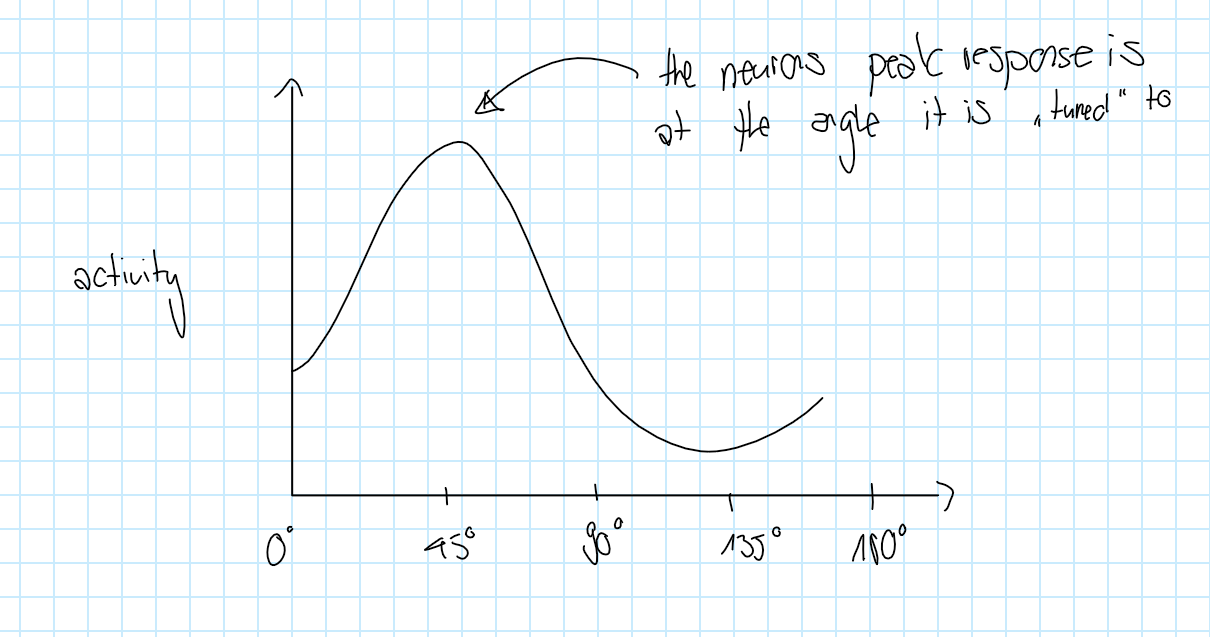
\includegraphics[width=0.5\textwidth]{assets/activity.png}
\caption{Neuron activity}
\end{figure}

\begin{figure}[H]
\centering
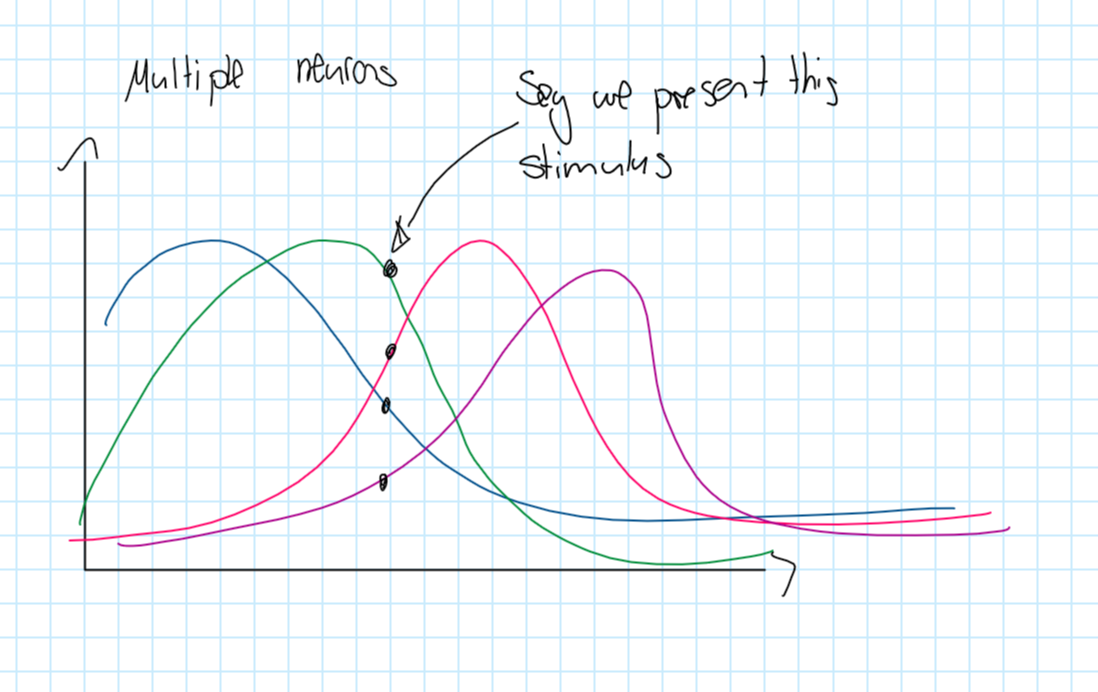
\includegraphics[width=0.5\textwidth]{assets/multipleActivity.png}
\caption{Multiple neuron activity}
\end{figure}

To read out a value, we look at the activities in the population.

\begin{figure}[H]
\centering
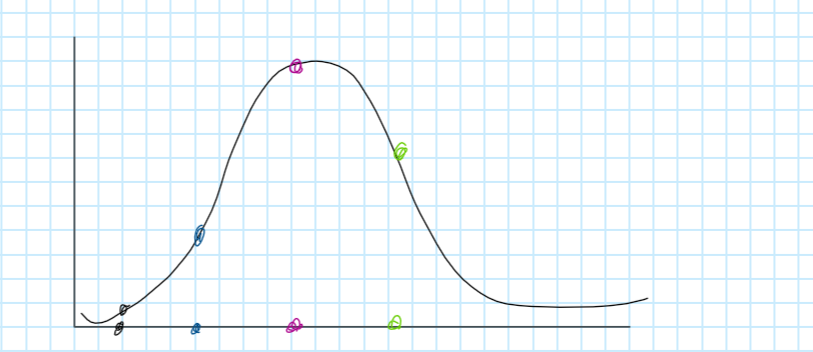
\includegraphics[width=0.5\textwidth]{assets/tunedActivity.png}
\caption{Tuned neuron activity}
\end{figure}

We plot each neuron at the position it is tuned to. The green neuron activity is always shown positioned at 170° because that is the angle it is tuned to.

Why are curves of a similar shape? Think of a 3D picture.

\begin{figure}[H]
\centering
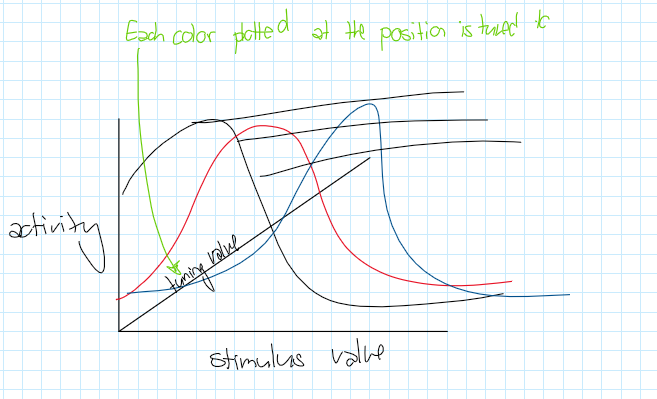
\includegraphics[width=0.5\textwidth]{assets/multipleGraph.png}
\caption{3D representation}
\end{figure}

Other neurons can reliably and accurately read out the value. Some neurons are tuned to values, with high firing rates at those values. Some neurons have a threshold, and as the stimulus passes, the threshold, the rate goes up.

\begin{figure}[H]
\centering
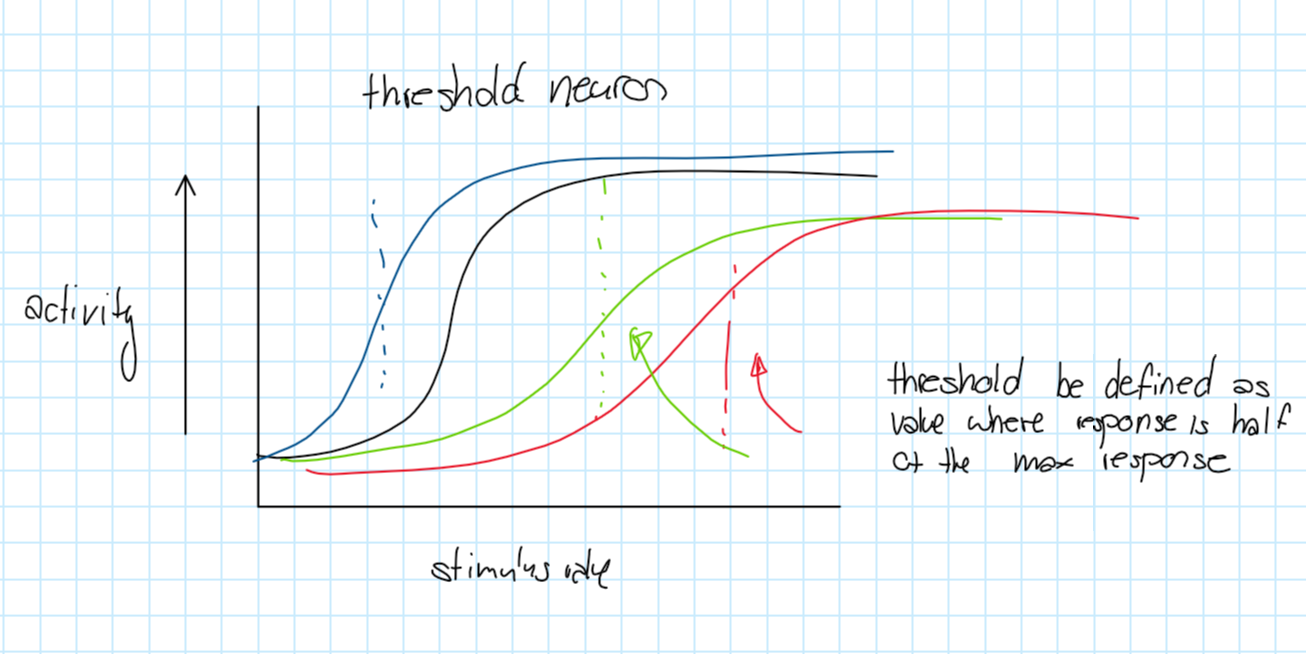
\includegraphics[width=0.5\textwidth]{assets/graphConversion.png}
\caption{Graph conversion}
\end{figure}

Again, easy for other neurons to read out robustly and accurately.

\begin{figure}[H]
\centering
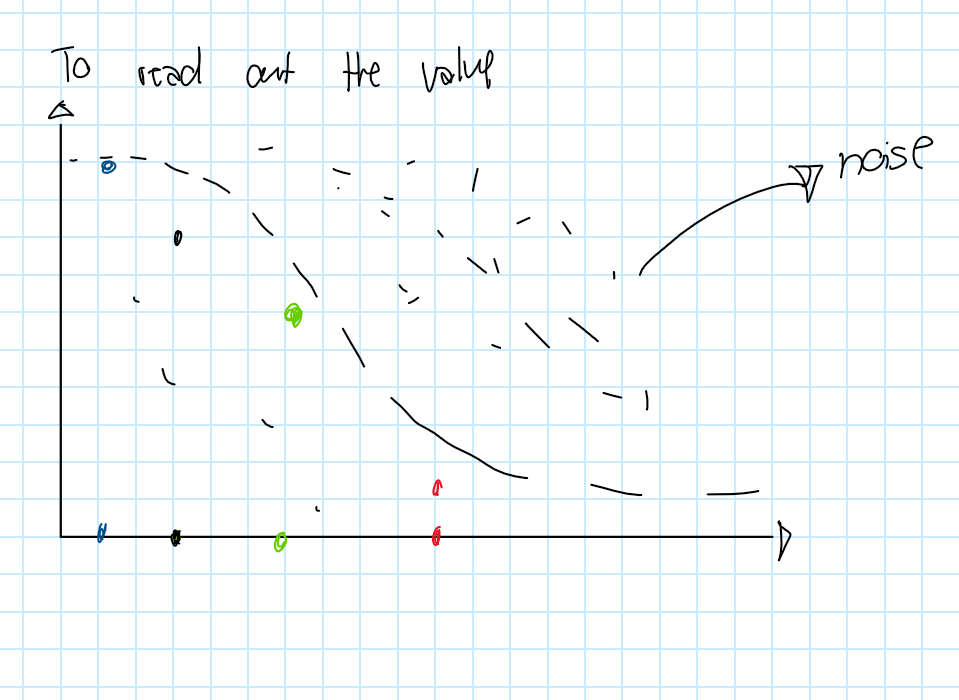
\includegraphics[width=0.5\textwidth]{assets/graphConversion2.png}
\caption{Graph conversion 2}
\end{figure}

Is it easy to convert between these formats?

\begin{figure}[H]
\centering
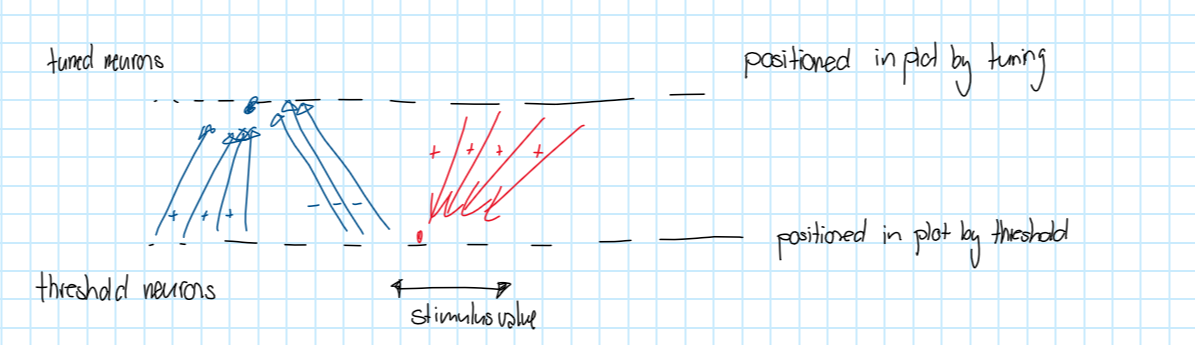
\includegraphics[width=0.5\textwidth]{assets/image.png}
\caption{Image}
\end{figure}

\begin{figure}[H]
\centering
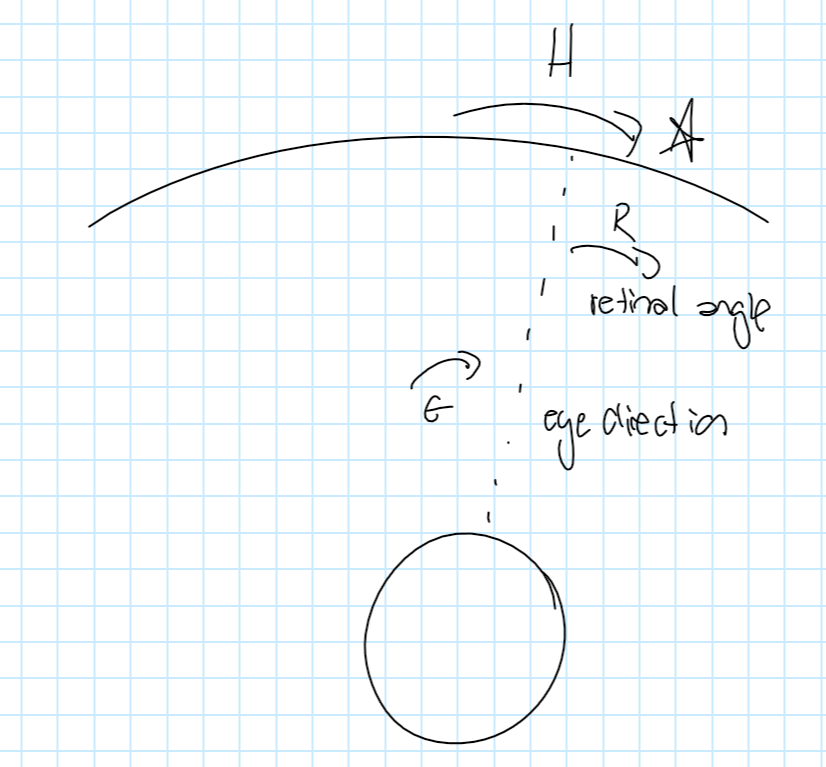
\includegraphics[width=0.5\textwidth]{assets/image-1.png}
\caption{Image 1}
\end{figure}

How can we compute something with this sort of data encoding? We'll use tuning-based units because threshold-based units only "work well" with scalars. In one dimension, the relationship is simple: \(H = E + R\).

\begin{figure}[H]
\centering
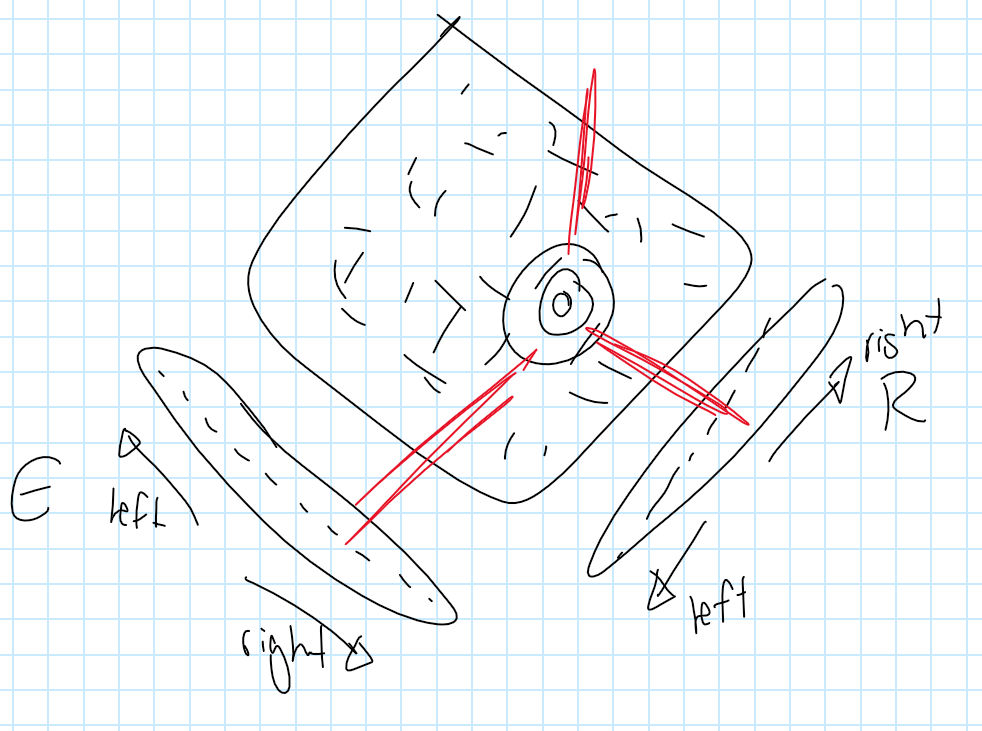
\includegraphics[width=0.5\textwidth]{assets/image-2.png}
\caption{Computational model}
\end{figure}

\section{Exam Questions}

\begin{enumerate}
    \item \textbf{Grid Cells}: Grid cells are types of neurons found in the brains of many animals, including humans, that allow for spatial navigation and are thought to form part of the brain's positioning system. These cells are located in the entorhinal cortex and exhibit a unique pattern of activity that corresponds to multiple, evenly spaced locations in an environment, forming a grid-like structure. This pattern helps in self-positioning and navigation by providing a metric for spatial coding. Understanding grid cells involves knowing how their firing patterns contribute to the neural code for representing space in the brain.

    \item \textbf{Brain Size Scaling with Species Size}: The relationship between brain size and the size of a species, also known as allometric scaling, is an important area of study in comparative neuroscience. Generally, brain size increases with body size, but not in a simple linear way; instead, it follows a power law where the exponent is less than one, indicating that larger animals have larger brains but not proportionally to their body size. This is sometimes expressed as the encephalization quotient (EQ), which measures brain mass relative to an expected value for a given body mass.

    \item \textbf{Perceptrons and XOR Function}: A perceptron is a simple linear classifier that can only solve linearly separable problems. The XOR function is not linearly separable, which means a single perceptron cannot compute an XOR function. However, a multi-layer network with at least one hidden layer (also known as a multi-layer perceptron) can solve the XOR problem by creating a non-linear decision boundary.

    \item \textbf{Convergence in Hopfield Networks}: A given state in a Hopfield network will converge to a stable state if it's close to one of the stored patterns (memories) or local minima of the energy function. To determine which of the four states will converge to a stable state, you would analyze the energy function of the Hopfield network and determine which states are local minima.

    \item \textbf{Output from an Integrate-and-Fire Circuit}: An integrate-and-fire neuron model is a simplified representation of a neuron that accumulates input signals until it reaches a threshold, at which point it 'fires' (generates an action potential) and then resets. The output of such a circuit is typically a series of spikes or action potentials over time.

    \item \textbf{Short-Term Plasticity vs Long-Term Potentiation}: Short-term plasticity refers to transient changes in synaptic strength that occur over a short period, such as facilitation or depression due to recent activity. Long-term potentiation (LTP), on the other hand, is a long-lasting increase in synaptic strength following high-frequency stimulation, which is a mechanism underlying learning and memory.

    \item \textbf{Tuning Curves (Population Codes)}: A tuning curve represents the response of a neuron to a range of stimuli, showing how the firing rate of the neuron changes with different stimulus values. It's an essential concept in understanding population coding, where the combined activity of multiple neurons with different tuning properties can encode complex information, such as sensory inputs.

    \item \textbf{Activation Levels from a 2D Stimuli Input}: The question likely refers to interpreting a heatmap or graph showing how a neuron's activation level varies with two-dimensional stimulus input. Areas of highest activation would correspond to the preferred stimulus of the neuron, while areas of lowest activation would correspond to non-preferred stimuli.

    \item \textbf{Action Potential Annihilation Due to Refractory Period}: The refractory period is the time immediately following an action potential during which a neuron is unable to fire another action potential. This refractory period prevents the backward propagation of the action potential and ensures unidirectional travel along an axon.

    \item \textbf{Cable Equation and EPSP Potential}: The cable equation describes how electrical signals decay as they travel through the dendrites and axons of neurons. An excitatory postsynaptic potential (EPSP) is a temporary increase in postsynaptic membrane potential due to the flow of positively charged ions into the cell. The potential is highest at the site of the synapse and decreases with distance from the point of synaptic contact due to the cable properties of the neuron.
\end{enumerate}

re $R$ is the gas constant, $T$ is the temperature in Kelvin,$z$ is the valence of the ion, $F$ is the Faraday constant, and $[\text{ion}]_{\text{outside}}$ and $[\text{ion}]_{\text{inside}}$ are the external and internal concentrations of the ion, respectively.

\subsubsection*{Graph of LTP Changes}
Long-term potentiation (LTP) is typically visualized by plotting the post-synaptic response strength over time. A normal graph of LTP would show a stable baseline of synaptic response followed by a sudden and sustained increase in response following a high-frequency stimulus. A modified graph might show a diminished LTP response, possibly due to pharmacological intervention, genetic modification, or pathology. Analyzing such graphs would involve noting differences in the magnitude, onset, and duration of LTP.

\subsubsection*{Injecting Two Currents at Both Ends}
When injecting two currents into the ends of a neuron, the interaction of the currents will depend on the neuron's properties, such as membrane resistance and capacitance. The currents will spread passively inside the neuron and decay over distance. The actual effect also depends on whether the currents are excitatory or inhibitory and their relative strengths and timings.

\subsubsection*{Reversal Potential of a Single Ion}
The reversal potential (also known as equilibrium potential) for a single ion can be calculated using the Nernst equation:
\[
E_{\text{ion}} = \frac{RT}{zF} \ln\left(\frac{[\text{ion}]_{\text{outside}}}{[\text{ion}]_{\text{inside}}}\right)
\]
where \(R\) is the gas constant, \(T\) is the temperature in Kelvin, \(z\) is the valence of the ion, \(F\) is the Faraday constant, and \([\text{ion}]_{\text{outside}}\) and \([\text{ion}]_{\text{inside}}\) are the external and internal concentrations of the ion, respectively.

\subsubsection*{Property About Brains}
Humans do not have the largest brains in absolute size—that distinction goes to larger animals like whales or elephants. However, humans do have a high encephalization quotient (EQ), which is a measure of brain size relative to what would be expected for an animal of our body size. Humans also do not have the most neurons; for instance, some species of whales have more neurons due to their larger brains. Brain size generally scales with body size, but not in a simple linear relationship.

\subsubsection*{Resting Potential and Reversal Potential}
The resting potential of a cell is closest to the reversal potential of the ion that has the highest permeability across the cell membrane, which is typically potassium (K\(^+\)). This is due to the fact that the resting membrane is most permeable to K\(^+\), and the movement of K\(^+\) ions out of the cell has the most significant effect on the resting potential.

\subsubsection*{Ion Flow During Resting/Polarization/Depolarization}
During the resting state, K\(^+\) ions flow out of the cell, and Na\(^+\) ions flow into the cell, but the K\(^+\) flow is dominant, keeping the membrane potential close to the K\(^+\) reversal potential. During depolarization, Na\(^+\) ions flow rapidly into the cell, making the inside more positive. During repolarization, K\(^+\) ions flow out of the cell, restoring the negative internal environment.

\subsubsection*{Electrical Synapses vs. Chemical Synapses}
Electrical synapses are direct connections between cells that allow for the rapid transfer of electrical signals via gap junctions. They are bidirectional and can synchronize the activity of connected neurons. Chemical synapses, on the other hand, use neurotransmitters to transfer signals from one neuron to another, are unidirectional, and have a synaptic delay. They are also modifiable, meaning they can be strengthened or weakened over time, which is the basis for learning and memory.

\subsubsection*{Loewi's Experiment}
Otto Loewi demonstrated chemical neurotransmission by showing that stimulating one frog's heart could release a substance (later identified as acetylcholine) that, when transferred to another frog's heart, slowed its rate. This experiment provided evidence that nerve impulses could affect heart rate through chemical means.

\subsubsection*{Properties of the PLA (Perceptron Learning Algorithm)}
The PLA is an algorithm used to train perceptrons. It iteratively adjusts the weights and bias of the perceptron based on its output errors, moving the decision boundary towards the optimal position that separates the classes in linearly separable data sets.

\subsubsection*{Hopfield Networks}
Hopfield networks have discrete-time dynamics with binary threshold units, are fully connected, and have symmetric weight matrices. They serve as associative memories by converging to stable states, which represent the memorized patterns.

\subsubsection*{Perceptrons vs. Logic Gates}
Perceptrons are a simple model of a neuron that can learn to make decisions by adjusting its weights in response to training data. Logic gates, however, are fixed-function devices that perform basic logical operations like AND, OR, and NOT without the ability to learn. Perceptrons can implement certain logic gates (like AND and OR for linearly separable patterns) but not others.

\subsection{Since this is a linear system, which of the following will always be true?}

\begin{enumerate}
    \item The weighting coefficients always lie on a straight line
      \begin{itemize}
        \item False
      \end{itemize}
    \item If you scale the input by a constant, the output will be scaled by the same constant
      \begin{itemize}
        \item True
      \end{itemize}
    \item The output of a sum of different inputs is equal to the sum of the outputs of each of the individual inputs
      \begin{itemize}
        \item True
      \end{itemize}
    \item The filter is a linear function of the input
      \begin{itemize}
        \item False
      \end{itemize}
\end{enumerate}

\subsection{Which of the following inputs might cause a linear system with a positive filter to predict a negative rate?}

\begin{enumerate}
    \item An input that slowly varies between a large positive value and a large negative value
      \begin{itemize}
        \item true
      \end{itemize}
    \item A positive input that decays to zero over time
    \item A positive input with a discontinuity
    \item None of these
\end{enumerate}



\end{document}
